% MAIN DOC
% Example for dissertation.sty
\documentclass[
  % Replace oneside by twoside if you are printing your thesis on both sides
  % of the paper, leave as is for single sided prints or for viewing on screen.
  % oneside,
  twoside=false,
  fontsize=12pt,% NewsGotT
  paper=a4,
  footinclude=true,
  headinclude=true,
  cleardoublepage=empty,
  headsepline=true,
  headheight=20pt,
  footheight=20pt,
  automark,
  markcase=upper,
  bibliography=totoc,
  %appendix=totoc
  %pagestyle=myheadings
  %footsepline=true,
]{scrbook}

% use the formatting style defined (this file should include all other packages)
%\usepackage{./sty/dissertation}% pdflatex
\usepackage{./sty/dissertation-xelatex}% xelatex

% fixing \vbox and \hbox underfull and overfull
% src: https://tex.stackexchange.com/a/387912
\raggedbottom%

%\addtokomafont{section}{\clearpage}
\addtokomafont{caption}{\small}

%this shall be the last thing in the acronym configuration!!
\makeglossaries%

%% **MORE INFO** %%
%to add the acronyms list add the following where you want to print it:
%\printglossary[type=\acronymtype]
%\clearpage
%\thispagestyle{empty}
%to use an acronym:
%\gls{qps}

% Reverse side notes
% How to generate 2 different files based on conditionals
% https://tex.stackexchange.com/a/220101
% see also makefile rule all-comm
\ifdef{\comm}{\reversemarginpar}

% ------------------------------------------------------------------------
% Title
\mytitle% defined in .sty file

% Glossaries & Acronyms
%\makeglossaries  %  either use this ...
%\makeindex	   % ... or this

% Define Acronyms
%%!TEX root = ../dissertation.tex
%
% here are the acronym entries
\newacronym{mei}{MEI}{Mestrado em Engenharia Inform\'{a}tica}
\newacronym{um}{UM}{Universidade do Minho}
\newacronym{di}{DI}{Departamento de Inform\'{a}tica}
%
\newacronym{qos}{QoS}{Quality of Service}
\newacronym{soa}{SOA}{Service Oriented Architecture}
%
\newacronym{oop}{OOP}{Object Oriented Programming}
\newacronym{oose}{OOSE}{Object Oriented Software Engineering}
\newacronym{omt}{OMT}{Object-Modeling Technique}
\newacronym{vdi}{VDI}{Verein Deutscher Ingenieure}
\newacronym{api}{API}{Application Programming Interface}
\newacronym{pwm}{PWM}{Pulse-Width Modulation}
\newacronym{ic}{IC}{Integrated Circuit}
\newacronym{ssr}{SSR}{Solid-State Relay}
%\newacronym{pid}{PID}{Proportional Integrative Derivative}
\newacronym{pci}{PCI}{Peripheral Component Interconnect}
\newacronym{pcb}{PCB}{Printed Circuit Board}
\newacronym{io}{I/O}{Input/Output}
%
% ========================== Article_Mach ========================
\newacronym{am}{AM}{Additive Manufacturing}
\newacronym{lbam}{LBAM}{Laser-based Additive Manufacturing}
\newacronym{fgm}{FGM}{Functionally Graded Material}
\newacronym{mmfgm}{MMFGM}{Multi-Material Functionally Graded Material}
\newacronym{mmam}{MMAM}{Multi-Material Additive Manufacturing}
\newacronym{oom}{OOM}{Object-Oriented Modelling}
\newacronym{uml}{UML}{Unified Modeling Language}
\newacronym{sls}{SLS}{Selective Laser Sintering}
\newacronym{slm}{SLM}{Selective Laser Melting}
\newacronym{mmsls}{MMSLS}{Multi-Material SLS}
\newacronym{mms}{MMS}{Multi-Material Sintering}
\newacronym{doe}{DOE}{Design Of Experiments}
\newacronym{ai}{AI}{Artificial Intelligence}
\newacronym{cad}{CAD}{Computer-Aided Design}
\newacronym{cae}{CAE}{Computer-Aided Engineering}
\newacronym{cam}{CAM}{Computer-Aided Manufacturing}
\newacronym{stl}{STL}{Standard Template Language}
\newacronym{amf}{AMF}{Additive Manufacturing File}
\newacronym{3mf}{3MF}{3D Manufacturing Format}
\newacronym{pov}{POV}{Persistence Of Vision}
\newacronym{dlp}{DLP}{Digital Light Projector}
\newacronym{tin}{TIN}{Triangular Irregular Network}
\newacronym{nc}{NC}{Numerical Control}
\newacronym{cnc}{CNC}{Computer Numerical Control}
\newacronym{svg}{SVG}{Scalable Vector Graphics}
\newacronym{html}{HTML}{Hypertext Markup Language}
\newacronym{xml}{XML}{eXtensible Markup Language}
\newacronym{gui}{GUI}{Graphical User Interface}
\newacronym{astm}{ASTM}{American Society for Testing and Materials}
\newacronym{fdm}{FDM}{Fused Deposition Material}
\newacronym{fff}{FFF}{Fused Filament Fabrication}
\newacronym{lom}{LOM}{Laminated Object Manufacturing}
\newacronym{pbf}{PBF}{Powder Bed Fusion}
\newacronym{ded}{DED}{Direct Energy Deposition}
\newacronym{dld}{DLD}{Direct Laser Deposition}
\newacronym{ebm}{EBM}{Electron Beam Melting}
% ================================================================
%
\newacronym{vm}{VM}{Virtual Machine}
\newacronym{lvm}{LVM}{Linux Virtual Machine}
\newacronym{usb}{USB}{Universal Serial Bus}
\newacronym{cli}{CLI}{Command Line Interface}
\newacronym{rtos}{RTOS}{Real-Time Operating System}
\newacronym{ui}{UI}{User Interface}
%
% Final report
\newacronym{rfcar}{RFCAR}{Radio Frequency Camera Assisted Rover}
\newacronym{qfd}{QFD}{Quality Function Deployment}
\newacronym{sig}{SIG}{Bluetooth Special Interest Group}
\newacronym{ble}{BLE}{Bluetooth Low---Energy}
\newacronym{iot}{IOT}{Internet of Things}
\newacronym{tcp}{TCP}{Transmission Control Protocol}
\newacronym{ip}{IP}{Internet Protocol}
\newacronym{tcp-ip}{TCP/IP}{Transmission Control Protocol/Internet Protocol}
\newacronym{hci}{HCI}{Host Controller Interface}
\newacronym{udp}{UDP}{User Datagram Protocol}
\newacronym{rfcomm}{RFCOMM}{Radio Frequency Communications}
\newacronym{l2cap}{L2CAP}{Logical Link Control and Adaptation Protocol}
\newacronym{acl}{ACL}{Asynchronous Connection-Oriented Logical}
\newacronym{sco}{SCO}{Synchronous Connection-Oriented}
\newacronym{psm}{PSM}{Protocol Service Multiplexers}
\newacronym{sdp}{SDP}{Service Device Protocol}
\newacronym{ipc}{IPC}{Inter-Process Communication}
%\newacronym{io}{I/O}{Input/Output}
\newacronym{gprs}{GPRS}{General Packet Radio Service}
\newacronym{gsm}{GSM}{Global System for Mobile Communications}
\newacronym{sms}{SMS}{Short Message Service}
\newacronym{lan}{LAN}{Local Area Network}
\newacronym{sgsn}{SGSN}{Serving GPRS Support Node}
\newacronym{ggsn}{GGSN}{Gateway GPRS Support Node}
\newacronym{ms}{MS}{Mobile Station}
\newacronym{me}{ME}{Mobile Equipment}
\newacronym{sim}{SIM}{Subscriber Identity Module}
\newacronym{dl}{DL}{downlink}
\newacronym{pdp}{PDP}{Packet Data Protocol}
\newacronym{at}{AT}{ATtention}
\newacronym{osi}{OSI}{Open Systems Interconnection}
\newacronym{wlan}{WLAN}{Wireless local Area Network}
\newacronym{os}{OS}{Operating System}
\newacronym{nvs}{NVS}{Navigation Virtual Subsystem}
\newacronym{rvvs}{RVVS}{Remote Vision Virtual Subsystem}
\newacronym{i2c}{I2C}{Inter-Integrated Circuit}
\newacronym{spi}{I2C}{Serial Peripheral Interface}
\newacronym{ide}{IDE}{Integrated Development Environment}
\newacronym{pc}{PC}{Personal Computer}
\newacronym{csi}{CSI}{Camera Serial Interface}
\newacronym{v4l}{V4L}{Video4Linux}
\newacronym{v4l2}{V4L2}{Video4Linux2}
\newacronym{sd}{SD}{Storage Disk}
\newacronym{ssh}{SSH}{Secure Shell}
\newacronym{scp}{SCP}{Secure Copy}
\newacronym{sftp}{SFTP}{Secure File Transfer Protocol}
\newacronym{gps}{GPS}{Global Positioning System}
%
%
% Hierarchical structure for MAC
\newglossaryentry{MAC}{name={MAC},description={\nopostdesc}}
\newacronym[parent=MAC]{mac1}{MAC}{Machine Address Code}
\newacronym[parent=MAC]{mac2}{MAC}{Media Access Control}
%
\newacronym{led}{LED}{Light Emitting Diode}
\newacronym{tv}{TV}{Television}
\newacronym{hw}{HW}{Hardware}
\newacronym{sw}{SW}{Software}
\newacronym{ir}{IR}{infrared}
\newacronym{lirc}{LIRC}{Linux Infrared Remote Control}
\newacronym{cots}{COTS}{Commercial off-the-shelf}
\newacronym{pca}{PCA}{Programmable Counter Array}
\newacronym{mcu}{MCU}{Micro Controller Unit}
\newacronym{cpu}{CPU}{Central Processing Unit}
\newacronym{gpu}{GPU}{Graphics Processing Unit}
\newacronym{isr}{ISR}{Interrupt Service Routine}
\newacronym{fifo}{FIFO}{First-In, First-Out}
\newacronym{dooh}{DOOH}{Digital Out-Of-Home}
\newacronym{bn}{BN}{Billions}
\newacronym{usd}{USD}{United States Dollar}
\newacronym{cagr}{CAGR}{Compound Annual Growth Rate}
\newacronym{rd}{R\&D}{Research and Development}
\newacronym{esrg}{ESRG}{Embedded Systems Research Group}
\newacronym{cps}{CPS}{Cyber---Physical Systems}
\newacronym{mdo}{MDO}{Marketing Digital Outdoor}
\newacronym{gif}{GIF}{Graphics Interchange Format}
\newacronym{mdo-rc}{MDO-RC}{MDO Remote Client}
\newacronym{mdo-rs}{MDO-RS}{MDO Remote Server}
\newacronym{mdo-l}{MDO-L}{MDO Local System}
\newacronym{db}{DB}{Database}
\newacronym{bsp}{BSP}{Board Support Package}
\newacronym{rdbms}{RDBMS}{Relational Database Management System}
\newacronym{dbms}{DBMS}{Database Management System}
\newacronym{cv}{CV}{Computer Vision}
\newacronym{soc}{SoC}{System-on-a-Chip}
\newacronym{ac}{AC}{Alternating Current}
\newacronym{dc}{DC}{Direct Current}
\newacronym{posix}{POSIX}{Portable Operating System Interface}
\newacronym{ocr}{OCR}{Optical Character Recognition}
\newacronym{cnn}{CNN}{Convolutional Neural Network}
\newacronym{hd}{HD}{High-Definition}
\newacronym{dpm}{DPM}{Deformable part models}
\newacronym{svm}{SVM}{Support Vector Machine}
\newacronym{acf}{ACF}{Aggregated channel feature}
\newacronym{hog}{HOG}{Histogram of Oriented Gradients}
\newacronym{ann}{ANN}{Artificial Neural Networks}
\newacronym{knn}{KNN}{K-nearest neighbor}
\newacronym{nb}{NB}{Naive Bayes}
\newacronym{roi}{ROI}{Region Of Interest}
\newacronym{sql}{SQL}{Structured Query Language}
\newacronym{er}{ER}{Entity-Relationship}
\newacronym{wal}{WAL}{Write-Ahead Log}
\newacronym{pgid}{PGID}{Process Group ID}
\newacronym{sid}{SID}{Session ID}
\newacronym{pid}{PID}{Process ID}
\newacronym{erd}{ERD}{Entities-Relationships diagram}
\newacronym{ddl}{DDL}{Data Definition Language}
\newacronym{dml}{DML}{Data Manipulation Language}
\newacronym{bsd}{BSD}{Berkeley Software Distribution}
\newacronym{pir}{PIR}{Passive Infrared}
\newacronym{mw}{MW}{Microwave}
\newacronym{mosfet}{MOSFET}{Metal Oxide Semiconductor Field-Effect Transistor}
\newacronym{fps}{FPS}{Frames per Second}
\newacronym{sdk}{SDK}{Software Development Kit}
\newacronym{http}{HTTP}{Hypertext Transfer Protocol}
\newacronym{rest}{REST}{Representation State Transfer}
\newacronym{json}{JSON}{Javascript Object Notation}
\newacronym{url}{URL}{Uniform Resource Locator}
% ========================== END ======================
%\glsaddall[types={\acronymtype}]

\begin{document}
	% Cover page ---------------------------------------
%	\umfrontcover%	
	\umtitlepage%
%
%% UNUSED - the title should be modified in \mytitle contained in *.sty file

% Title
\titleA{First Part of Title}
\titleB{Second Part of Title} % (if any)
\subtitleA{First Part of Subtitle}
\subtitleB{Second part of Subtitle} % (if any)

% Author
\author{Author of the Thesis}

% Supervisor(s)
\supervisor{The Supervisor of the thesis}
\cosupervisor{The cosupervisor of the thesis}

% University (uncomment if you need to change default values)
% \def\school{Escola de Engenharia}
% \def\department{Departamento de Inform\'{a}tica}
% \def\university{Universidade do Minho}
% \def\masterdegree{Computer Science}

% Date
\date{\myear} % change to text if date is not today

% Keywords
%\keywords{master thesis}

% Glossaries & Acronyms
%\makeglossaries  %  either use this ...
%\makeindex	   % ... or this

% Define Acronyms
%%!TEX root = ../dissertation.tex
%
% here are the acronym entries
\newacronym{mei}{MEI}{Mestrado em Engenharia Inform\'{a}tica}
\newacronym{um}{UM}{Universidade do Minho}
\newacronym{di}{DI}{Departamento de Inform\'{a}tica}
%
\newacronym{qos}{QoS}{Quality of Service}
\newacronym{soa}{SOA}{Service Oriented Architecture}
%
\newacronym{oop}{OOP}{Object Oriented Programming}
\newacronym{oose}{OOSE}{Object Oriented Software Engineering}
\newacronym{omt}{OMT}{Object-Modeling Technique}
\newacronym{vdi}{VDI}{Verein Deutscher Ingenieure}
\newacronym{api}{API}{Application Programming Interface}
\newacronym{pwm}{PWM}{Pulse-Width Modulation}
\newacronym{ic}{IC}{Integrated Circuit}
\newacronym{ssr}{SSR}{Solid-State Relay}
%\newacronym{pid}{PID}{Proportional Integrative Derivative}
\newacronym{pci}{PCI}{Peripheral Component Interconnect}
\newacronym{pcb}{PCB}{Printed Circuit Board}
\newacronym{io}{I/O}{Input/Output}
%
% ========================== Article_Mach ========================
\newacronym{am}{AM}{Additive Manufacturing}
\newacronym{lbam}{LBAM}{Laser-based Additive Manufacturing}
\newacronym{fgm}{FGM}{Functionally Graded Material}
\newacronym{mmfgm}{MMFGM}{Multi-Material Functionally Graded Material}
\newacronym{mmam}{MMAM}{Multi-Material Additive Manufacturing}
\newacronym{oom}{OOM}{Object-Oriented Modelling}
\newacronym{uml}{UML}{Unified Modeling Language}
\newacronym{sls}{SLS}{Selective Laser Sintering}
\newacronym{slm}{SLM}{Selective Laser Melting}
\newacronym{mmsls}{MMSLS}{Multi-Material SLS}
\newacronym{mms}{MMS}{Multi-Material Sintering}
\newacronym{doe}{DOE}{Design Of Experiments}
\newacronym{ai}{AI}{Artificial Intelligence}
\newacronym{cad}{CAD}{Computer-Aided Design}
\newacronym{cae}{CAE}{Computer-Aided Engineering}
\newacronym{cam}{CAM}{Computer-Aided Manufacturing}
\newacronym{stl}{STL}{Standard Template Language}
\newacronym{amf}{AMF}{Additive Manufacturing File}
\newacronym{3mf}{3MF}{3D Manufacturing Format}
\newacronym{pov}{POV}{Persistence Of Vision}
\newacronym{dlp}{DLP}{Digital Light Projector}
\newacronym{tin}{TIN}{Triangular Irregular Network}
\newacronym{nc}{NC}{Numerical Control}
\newacronym{cnc}{CNC}{Computer Numerical Control}
\newacronym{svg}{SVG}{Scalable Vector Graphics}
\newacronym{html}{HTML}{Hypertext Markup Language}
\newacronym{xml}{XML}{eXtensible Markup Language}
\newacronym{gui}{GUI}{Graphical User Interface}
\newacronym{astm}{ASTM}{American Society for Testing and Materials}
\newacronym{fdm}{FDM}{Fused Deposition Material}
\newacronym{fff}{FFF}{Fused Filament Fabrication}
\newacronym{lom}{LOM}{Laminated Object Manufacturing}
\newacronym{pbf}{PBF}{Powder Bed Fusion}
\newacronym{ded}{DED}{Direct Energy Deposition}
\newacronym{dld}{DLD}{Direct Laser Deposition}
\newacronym{ebm}{EBM}{Electron Beam Melting}
% ================================================================
%
\newacronym{vm}{VM}{Virtual Machine}
\newacronym{lvm}{LVM}{Linux Virtual Machine}
\newacronym{usb}{USB}{Universal Serial Bus}
\newacronym{cli}{CLI}{Command Line Interface}
\newacronym{rtos}{RTOS}{Real-Time Operating System}
\newacronym{ui}{UI}{User Interface}
%
% Final report
\newacronym{rfcar}{RFCAR}{Radio Frequency Camera Assisted Rover}
\newacronym{qfd}{QFD}{Quality Function Deployment}
\newacronym{sig}{SIG}{Bluetooth Special Interest Group}
\newacronym{ble}{BLE}{Bluetooth Low---Energy}
\newacronym{iot}{IOT}{Internet of Things}
\newacronym{tcp}{TCP}{Transmission Control Protocol}
\newacronym{ip}{IP}{Internet Protocol}
\newacronym{tcp-ip}{TCP/IP}{Transmission Control Protocol/Internet Protocol}
\newacronym{hci}{HCI}{Host Controller Interface}
\newacronym{udp}{UDP}{User Datagram Protocol}
\newacronym{rfcomm}{RFCOMM}{Radio Frequency Communications}
\newacronym{l2cap}{L2CAP}{Logical Link Control and Adaptation Protocol}
\newacronym{acl}{ACL}{Asynchronous Connection-Oriented Logical}
\newacronym{sco}{SCO}{Synchronous Connection-Oriented}
\newacronym{psm}{PSM}{Protocol Service Multiplexers}
\newacronym{sdp}{SDP}{Service Device Protocol}
\newacronym{ipc}{IPC}{Inter-Process Communication}
%\newacronym{io}{I/O}{Input/Output}
\newacronym{gprs}{GPRS}{General Packet Radio Service}
\newacronym{gsm}{GSM}{Global System for Mobile Communications}
\newacronym{sms}{SMS}{Short Message Service}
\newacronym{lan}{LAN}{Local Area Network}
\newacronym{sgsn}{SGSN}{Serving GPRS Support Node}
\newacronym{ggsn}{GGSN}{Gateway GPRS Support Node}
\newacronym{ms}{MS}{Mobile Station}
\newacronym{me}{ME}{Mobile Equipment}
\newacronym{sim}{SIM}{Subscriber Identity Module}
\newacronym{dl}{DL}{downlink}
\newacronym{pdp}{PDP}{Packet Data Protocol}
\newacronym{at}{AT}{ATtention}
\newacronym{osi}{OSI}{Open Systems Interconnection}
\newacronym{wlan}{WLAN}{Wireless local Area Network}
\newacronym{os}{OS}{Operating System}
\newacronym{nvs}{NVS}{Navigation Virtual Subsystem}
\newacronym{rvvs}{RVVS}{Remote Vision Virtual Subsystem}
\newacronym{i2c}{I2C}{Inter-Integrated Circuit}
\newacronym{spi}{I2C}{Serial Peripheral Interface}
\newacronym{ide}{IDE}{Integrated Development Environment}
\newacronym{pc}{PC}{Personal Computer}
\newacronym{csi}{CSI}{Camera Serial Interface}
\newacronym{v4l}{V4L}{Video4Linux}
\newacronym{v4l2}{V4L2}{Video4Linux2}
\newacronym{sd}{SD}{Storage Disk}
\newacronym{ssh}{SSH}{Secure Shell}
\newacronym{scp}{SCP}{Secure Copy}
\newacronym{sftp}{SFTP}{Secure File Transfer Protocol}
\newacronym{gps}{GPS}{Global Positioning System}
%
%
% Hierarchical structure for MAC
\newglossaryentry{MAC}{name={MAC},description={\nopostdesc}}
\newacronym[parent=MAC]{mac1}{MAC}{Machine Address Code}
\newacronym[parent=MAC]{mac2}{MAC}{Media Access Control}
%
\newacronym{led}{LED}{Light Emitting Diode}
\newacronym{tv}{TV}{Television}
\newacronym{hw}{HW}{Hardware}
\newacronym{sw}{SW}{Software}
\newacronym{ir}{IR}{infrared}
\newacronym{lirc}{LIRC}{Linux Infrared Remote Control}
\newacronym{cots}{COTS}{Commercial off-the-shelf}
\newacronym{pca}{PCA}{Programmable Counter Array}
\newacronym{mcu}{MCU}{Micro Controller Unit}
\newacronym{cpu}{CPU}{Central Processing Unit}
\newacronym{gpu}{GPU}{Graphics Processing Unit}
\newacronym{isr}{ISR}{Interrupt Service Routine}
\newacronym{fifo}{FIFO}{First-In, First-Out}
\newacronym{dooh}{DOOH}{Digital Out-Of-Home}
\newacronym{bn}{BN}{Billions}
\newacronym{usd}{USD}{United States Dollar}
\newacronym{cagr}{CAGR}{Compound Annual Growth Rate}
\newacronym{rd}{R\&D}{Research and Development}
\newacronym{esrg}{ESRG}{Embedded Systems Research Group}
\newacronym{cps}{CPS}{Cyber---Physical Systems}
\newacronym{mdo}{MDO}{Marketing Digital Outdoor}
\newacronym{gif}{GIF}{Graphics Interchange Format}
\newacronym{mdo-rc}{MDO-RC}{MDO Remote Client}
\newacronym{mdo-rs}{MDO-RS}{MDO Remote Server}
\newacronym{mdo-l}{MDO-L}{MDO Local System}
\newacronym{db}{DB}{Database}
\newacronym{bsp}{BSP}{Board Support Package}
\newacronym{rdbms}{RDBMS}{Relational Database Management System}
\newacronym{dbms}{DBMS}{Database Management System}
\newacronym{cv}{CV}{Computer Vision}
\newacronym{soc}{SoC}{System-on-a-Chip}
\newacronym{ac}{AC}{Alternating Current}
\newacronym{dc}{DC}{Direct Current}
\newacronym{posix}{POSIX}{Portable Operating System Interface}
\newacronym{ocr}{OCR}{Optical Character Recognition}
\newacronym{cnn}{CNN}{Convolutional Neural Network}
\newacronym{hd}{HD}{High-Definition}
\newacronym{dpm}{DPM}{Deformable part models}
\newacronym{svm}{SVM}{Support Vector Machine}
\newacronym{acf}{ACF}{Aggregated channel feature}
\newacronym{hog}{HOG}{Histogram of Oriented Gradients}
\newacronym{ann}{ANN}{Artificial Neural Networks}
\newacronym{knn}{KNN}{K-nearest neighbor}
\newacronym{nb}{NB}{Naive Bayes}
\newacronym{roi}{ROI}{Region Of Interest}
\newacronym{sql}{SQL}{Structured Query Language}
\newacronym{er}{ER}{Entity-Relationship}
\newacronym{wal}{WAL}{Write-Ahead Log}
\newacronym{pgid}{PGID}{Process Group ID}
\newacronym{sid}{SID}{Session ID}
\newacronym{pid}{PID}{Process ID}
\newacronym{erd}{ERD}{Entities-Relationships diagram}
\newacronym{ddl}{DDL}{Data Definition Language}
\newacronym{dml}{DML}{Data Manipulation Language}
\newacronym{bsd}{BSD}{Berkeley Software Distribution}
\newacronym{pir}{PIR}{Passive Infrared}
\newacronym{mw}{MW}{Microwave}
\newacronym{mosfet}{MOSFET}{Metal Oxide Semiconductor Field-Effect Transistor}
\newacronym{fps}{FPS}{Frames per Second}
\newacronym{sdk}{SDK}{Software Development Kit}
\newacronym{http}{HTTP}{Hypertext Transfer Protocol}
\newacronym{rest}{REST}{Representation State Transfer}
\newacronym{json}{JSON}{Javascript Object Notation}
\newacronym{url}{URL}{Uniform Resource Locator}
% ========================== END ======================
%\glsaddall[types={\acronymtype}]



\ummetadata % add metadata to the document (author, publisher, ...)

%\maketitle % should use a customized title creation
% see: https://en.wikibooks.org/wiki/LaTeX/Title_Creation
  % Add dedication
%  %\chapter*{Dedication}
% src: https://tex.stackexchange.com/a/167529
% see also: .sty file (lines 297-309)
\begin{dedicat}
  %\usefont{T1}{LobsterTwo-LF}{bx}{it}
  % src: https://en.wikibooks.org/wiki/LaTeX/Fonts
  \rmfamily
  {\Large To my parents,}\\
  {\large for always pushing me forward.}
  \par   %% or a blank line
  \vspace{4\baselineskip}
  
  \normalfont
  \emph{"Wir m{\"u}ssen wissen,\\ 
  Wir werden wissen"}\\
  \vspace{\baselineskip}
  David Hilbert, 1930

\end{dedicat}

%%
%% ----------License------
%  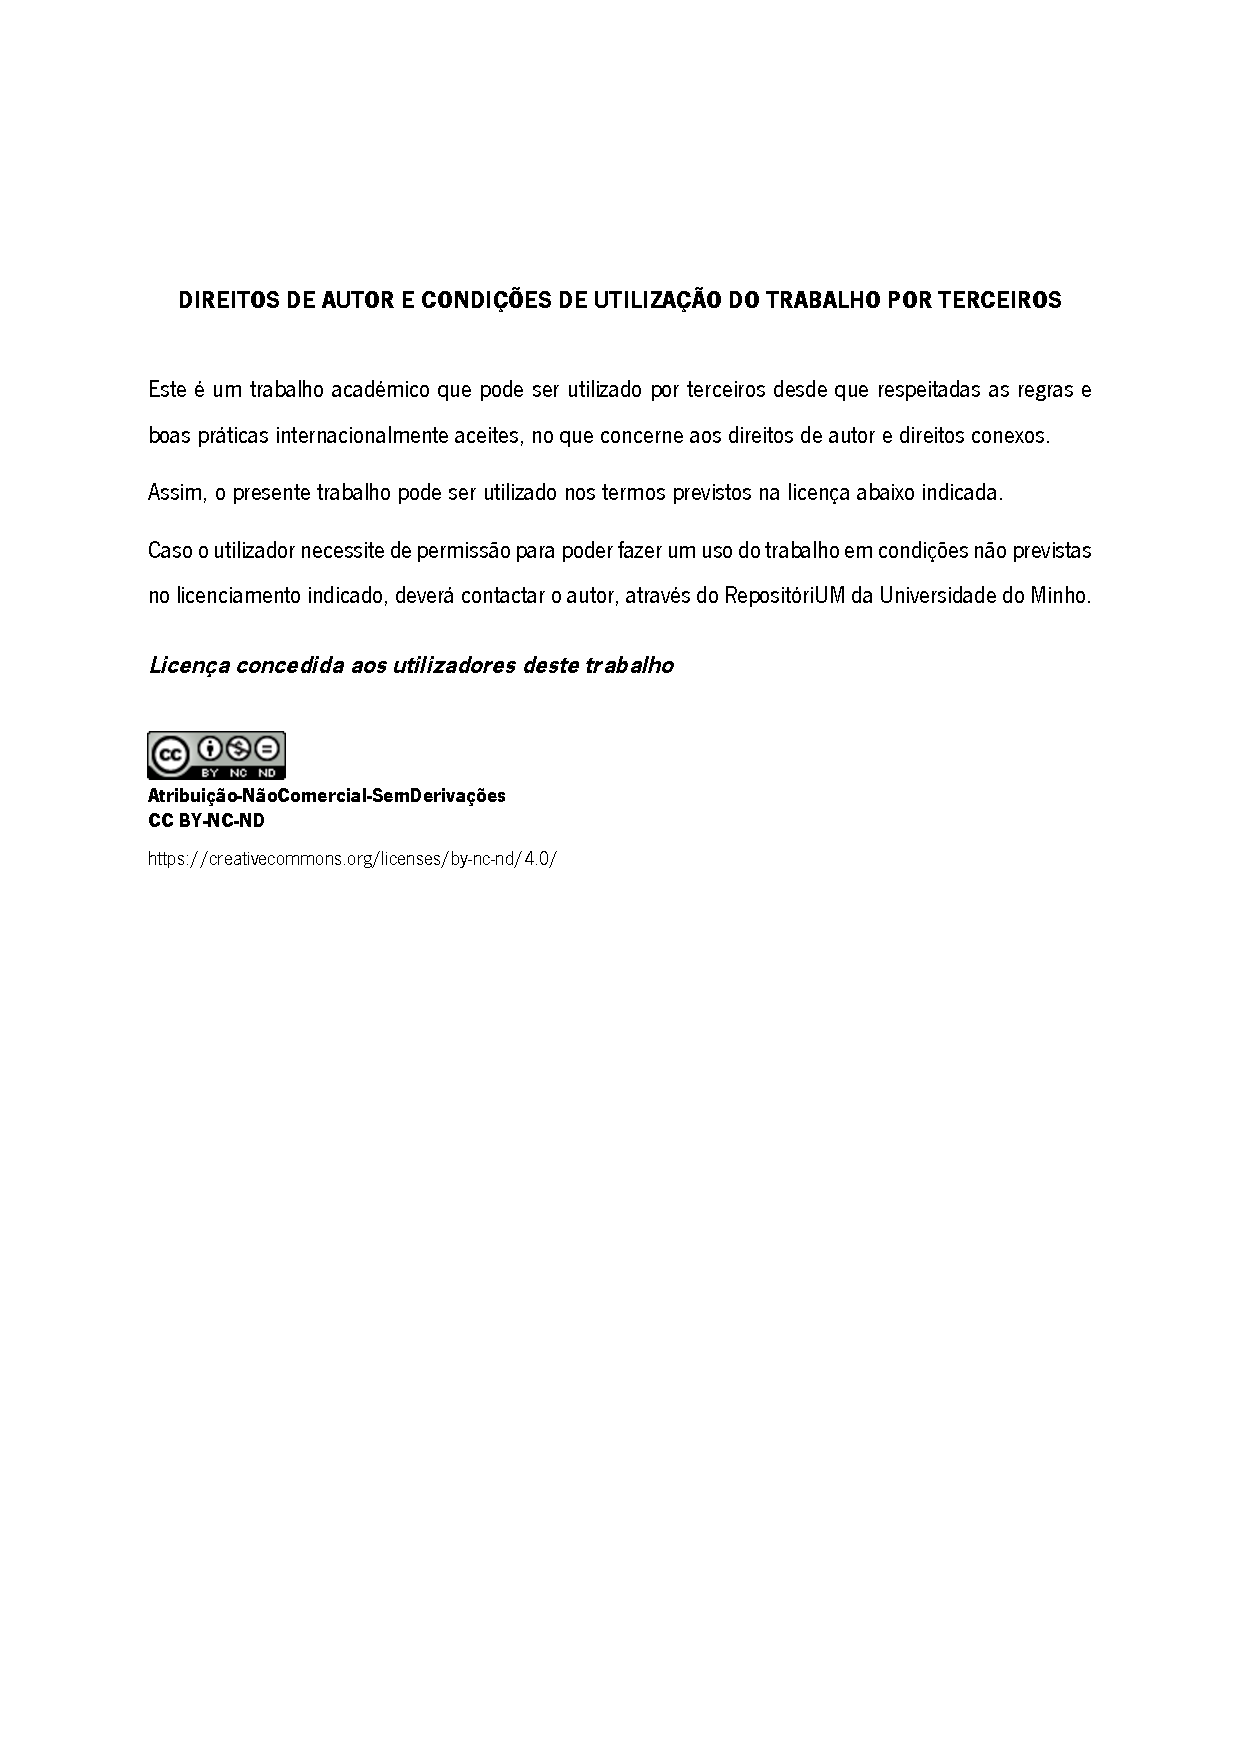
\includepdf[pages=-]{anexo3-license}
%  \cleardoublepage%
%%---------------------
%	% Add acknowledgements ----------------------------
%  \chapter*{Acknowledgements}
First and foremost, I would like to thank...
%%% Local Variables:
%%% mode: latex
%%% TeX-master: "../../dissertation"
%%% End:

%  %\chapter*{Acknowledgements}
%  %	Write acknowledgements here
%  \cleardoublepage%
%%---------------------
%  %
%  \KOMAoption{fontsize}{11.5pt}%
%	% Add abstracts (en,pt) ---------------------------
%  \chapter*{Abstract}
Functional design is the desirable and most sustainable method to design
products: by adding the material only where is strictly required to perform its
function, the resources usage is optimized, especially materials and
energy. However, functional design may dictate the usage of several materials or a combination of them to fulfill its goal, which is hindered by the
current manufacturing methodologies. An example of a class of
products where functional design is key is biomedical implants, like the hip implant.

% Keywords
\keywords{functional design, multimaterial, laser based additive manufacturing}
%%% Local Variables:
%%% mode: latex
%%% TeX-master: "../../dissertation"
%%% End:

%  %\chapter*{Abstract}
%	%Write abstract here (en) or import corresponding file	
%  \cleardoublepage%
%%
%  \KOMAoption{fontsize}{11pt}%
%  \chapter*{Resumo}
\selectlanguage{portuguese}%
O design funcional é o método mais desejável e sustentável de projetar
produtos: adicionando material somente é estritamente necessário para
a sua função, o uso de recursos é otimizado, especialmente materiais e

\keywordspt{design funcional, multimaterial, manufatura aditiva baseada em laser}
\selectlanguage{english}%
%%% Local Variables:
%%% mode: latex
%%% TeX-master: "../../dissertation"
%%% End:

%  %\chapter*{Resumo}
%	%Escrever aqui resumo (pt), ou importar respectivo ficheiro,
%  \cleardoublepage%
	% Summary Lists ------------------------------------
  % add toc and lists to TOC
  % src: https://tex.stackexchange.com/a/74440
%  \KOMAoption{fontsize}{12pt}%
  % TOC
  \phantomsection%
  \addcontentsline{toc}{chapter}{Contents}
  \tableofcontents%
  \cleardoublepage%
  % List of Figs
  \phantomsection%
  \addcontentsline{toc}{chapter}{List of Figures}
  \listoffigures%
  \cleardoublepage%
  % List of Tables
%  \phantomsection%
%  \addcontentsline{toc}{chapter}{List of Tables}
%  \listoftables
%  \cleardoublepage%
  % List of listings
  \phantomsection%
  \addcontentsline{toc}{chapter}{List of Listings}
  \lstlistoflistings%
  \cleardoublepage%
  % list of Acronyms
  \phantomsection%
  \addcontentsline{toc}{chapter}{List of Abbreviations}
  \listofacronyms%
  \cleardoublepage%
    %\printglossary[type=\acronymtype]%
    %\printglossary[type=\acronymtype]%
 %   \listofabbreviations%
  % List of symbols
  \phantomsection%
  \addcontentsline{toc}{chapter}{List of Symbols}
  \listofsymbols%
  \cleardoublepage%
%
	\thispagestyle{empty}
  %\newpage
	\pagenumbering{arabic}
  %\newpage
  %\setcounter{page}{0}
  %\pagenumbering{arabic}
  %\setcounter{page}{1}
 % 
  % making chapter pages with no header and footer
  \renewcommand*{\chapterpagestyle}{empty}
  %-------------- MAIN BODY CHAPTERS----------------------------------
  % Include the other files (\include adds a blank page between files)
  % - does not need the file extension
%  \KOMAoption{fontsize}{12pt}%
  \setlength{\unitlength}{1mm}
  %% 1,5 line spacing
  \renewcommand{\baselinestretch}{1.5}
%
  % For VIM to recognize the document syntax \begin{document} and \end{document}
% - However, the compilation will fail!! So don't forget to comment the
%   directives before compiling!!'
%
%\begin{document}
%
% CHAPTER - Introduction -------------------------
\chapter{Introduction}%
\label{ch:introduction}
The present work illustrates the application of the project meant to do for the course of Embedded Systems, required from the professors from \gls{esrg}.
This type of project begins with the establishment of what type of prototype do the students propose to do, followed for its implementation. This implementation needs to follow all the steps of the Waterfall Model in order to give students the capability to work the best way possible, either in group or in solo.

It should be noted, however, that there are some requirements and constraints gave by the professors which means that not everything is decided by the students. 
To have the capability of bypass them is one of the main characteristics of attending and working in engineering.
%
%  \vspace{-5mm}
  %
\section{Problem statement}%
\label{sec:prob-stat}
%The first step of the project is to clearly define the problem, as a result of
%the contract established between the client and the project team, yielding, in
%this case, the following project statement:
%
%``Design a remote control with three buttons that can
%remotely control the television (TV). It should be very
%light, powered by batteries and controls your TV via an
%infrared emitter. The TV has a built-in infrared receiver. A
%button on the remote control switches the TV on/off and
%will be labeled with the word "Power". The other two
%buttons are used to scroll up/down and select the available
%channels and they are labeled with the arrows up/down.''

%COVID pandemics presented a landmark on human interaction, greatly reducing the
%contact between people and surfaces. Thus, it is an imperative to provide people
%with contactless interfaces for everyday tasks. People redefined their
%purchasing behaviors, leading to a massive growth of the online
%shopping. However, some business sectors, like clothing or perfumes, cannot
%provide the same user experience when moving online.
%Therefore, one proposes to close that gap by providing a marketing digital
%outdoor for brands to advertise and gather customers with contactless
%interaction.
%
%Scenting marketing is a great approach to draw people into stores.
%Olfactory sense is the fastest way to the brain, thus, providing an exceptional
%opportunity for marketing~\cite{news-harvard} --- ``75\% of the emotions we generate on a daily basis are affected by smell. Next
%to sight, it is the most important sense we have''~\cite{lindstrom2006brand}.
%
%Combining that with additional stimuli, like sight and sound, can
%significantly boost the marketing outcome. Brands can buy advertisement space
%and time, selecting the videoclips to be displayed and the fragrance to be
%used at specific times, drawing the customers into their stores.
%
%Marketing also leverages from better user experience, thus, user interaction is
%a must-have, providing the opportunity to interact with the customer. In this
%sense, when users approach the outdoor a gesture-based interface will be
%provided for a brand immersive experience, where the user can take pictures or
%create GIFs with brand specific image filters and share them through their
%social media, with the opportunity to gain several benefits.

The first step of the project is to clearly define the problem, taking into
consideration the problem's context and motivation and exploiting the market opportunities.

\emph{The project consists of a \gls{mdo} with sound and
video display, and fragrance emission selected by the brands, providing a gesture-based interface for
user interaction to create pictures and \gls{gif}s, brand-specific, and share them on
social media.} It is comprised of several modes:
\begin{item-c}
\item \emph{normal mode (advertisement mode)}: the \gls{mdo} will provide
  sound, video and fragrance outputs.
\item \emph{interaction mode}: When a user approaches, the \gls{mdo} it will
go into interaction mode, turning on and displaying the camera feed and waiting
for recognizable gestures to provide additional functionalities, such as
brand-specific image filters.
\item \emph{sharing mode}: after a user take a picture or create a \gls{gif}, it
  can share it across social media.
\end{item-c}

Brands can buy advertisement space and time, selecting the videoclips to be
displayed and the fragrance to be used at specific times, drawing the customers
into their stores. Customers can be captivated by the combination of sensorial
stimuli, the gesture-based interaction, the immersive user experience provided
by the brands --- feeling they belong in a TV advertisement, and the opportunity
to gain several benefits, e.g., discount coupons.
%%% Local Variables:
%%% mode: latex
%%% TeX-master: "../../../dissertation"
%%% End:

\section{Context and motivation}
\label{sec:context-motivation}


%%% Local Variables:
%%% mode: latex
%%% TeX-master: "../../../dissertation"
%%% End:

\section{Market research}
\label{sec:market-research}
A Digital Outdoor is essentially a traditional outdoor advertising powered up by technology. 
The pros of a digital outdoor compared to a traditional one is mostly the way that it captivates the attention of consumers in a more dynamic way. 
It can also change its advertisement according to certain conditions, such as
weather and/or time. Some researches tells that the British public sees over 1.1
\gls{bn} digital outdoor advertisements over a week~\cite{digital-outdoor}, which can tell how much digital marketing is valued nowadays.

When talking about numbers, ``At the end of 2020, despite the Covid wipeout, the \gls{dooh} market was estimated to be worth \$41.06 \gls{bn}, but by 2026, nearly two out of three (65\%) advertising executives predict this will rise to between \$50 \gls{bn} and \$55 \gls{bn}. 
A further 16\% expect it to be worth between \$55 \gls{bn} and \$60 \gls{bn}, and 14\% estimate it will be even bigger''~\cite{outdoor-market}.

\begin{figure}[htb!]
\centering
    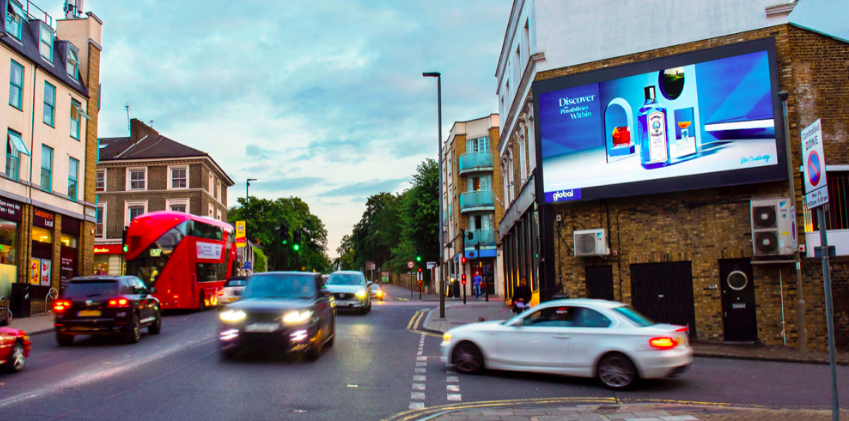
\includegraphics[width=0.7\columnwidth]{./img/DigitalOutdoor.png}
  \caption{Example of a Digital Outdoor, withdrawn from~\cite{digital-outdoor}}%
\label{fig:dig-outdoor}
\end{figure}

Scent market is the art of taking a company's brand identity, marketing messages, target audience and creating a scent that amplifies these values. 
That's because ``a scent has the ability to influence behavior and trigger memories almost instantaneously. When smell is combined with other marketing cues, it can amplify a brand experience and establish a long lasting connection with consumers''~\cite{scent-market}.

Ambient scent uses fragrance to enhance the experience of consumers with different purposes, whereas scents in scent branding are unique to each company's identity.
According to a Samsung study: ``when consumers were exposed to a company scent, shopping time was increased by 26\% and they visited three times more product categories'' ~\cite{scent-stats}.
Also, ``the digital scent technology market is expected to grow from \$1.0 \gls{bn} in 2021 to \$1.5 \gls{bn} by 2026, at a \gls{cagr} of 9.2\%.''~\cite{scent-money}.

\begin{figure}[htb!]
\centering
    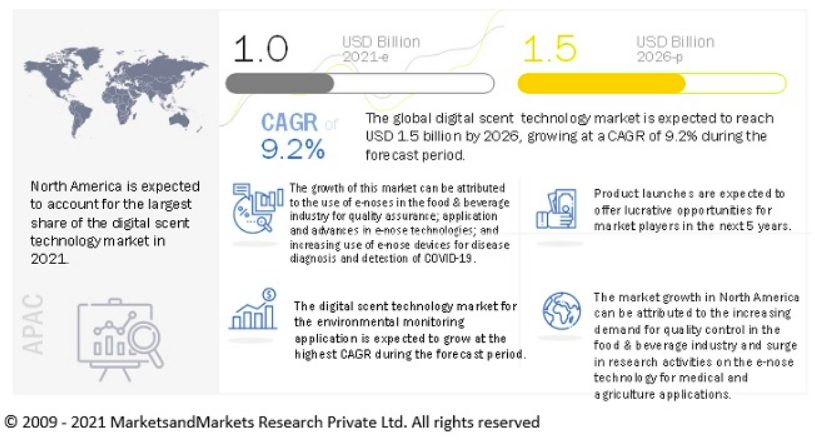
\includegraphics[width=0.9\columnwidth]{./img/scentstats.png}
  \caption{Attractive Opportunities in the Digital Scent Technology Market, withdrawn from~\cite{scent-money}}%
\label{fig:scent-stat}
\end{figure}

The market growth can be attributed to several factors, such as expanding application and advancements in e-nose technologies, increasing use of e-nose devices for disease diagnostic applications, emerging \gls{rd} activities to invent e-nose to sniff out COVID-19, and rising use of e-nose in food industry for quality assurance in production, storage, and display.

% Remote material (side by side)
%\begin{figure}[htb!]
%  \centering
  %
%  \begin{subfigure}{.4\textwidth}
%  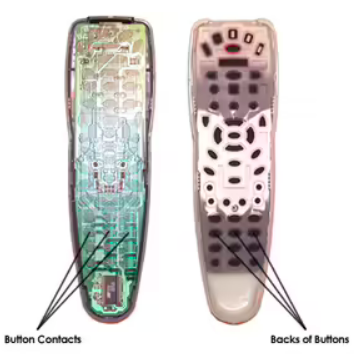
\includegraphics[width=\textwidth]{img/remotematerial1.png}%
  %\caption{KUKA's original position}%
  %\label{fig:ptp-test-orig}
%\end{subfigure}
%
 % \begin{subfigure}{.4\textwidth}
  %  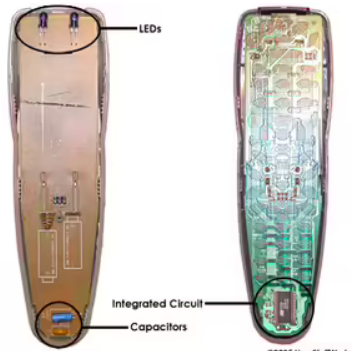
\includegraphics[width=\textwidth]{img/remotematerial2.png}%
%  \caption{KUKA's final position}%
%  \label{fig:ptp-test-final}
%\end{subfigure}
%
%  \caption{TV Remote control bill of materials, withdrawn from~\cite{remotematerial}}%
%  \label{fig:remotemat}
%\end{figure}
%

%%% Local Variables:
%%% mode: latex
%%% TeX-master: "../../../dissertation"
%%% End:

\section{Project goals}%
\label{sec:project-goals}
The project aims to develop a \gls{cps} for multi-sensorial marketing with
contactless user interaction. The key goals identified and the respective path
to attain them are:
\begin{enum-c}
\item \emph{devise a device with audio and video outputs, as well as fragrance
    diffusion}: understand audio and video streaming and study fragrance
  nebulizer technologies.
\item \emph{create a contactless user interface based on gestures through
    computer vision}: identify user gestures through computer vision and match them to interface
  callbacks; a virtual keyboard may be required for user input.
\item \emph{devise a distributed architecture to convey brand advertisement
  information to the local device}: understand distributed architectures and
apply them for optimal data flow; create a remote client-server model to convey
information from the brands to the device through remote cloud database
services; devise adequate data frames to convey information to the local device;
create a local server to respond to the remote server requests.
\item \emph{apply facial recognition to the camera feed and subsequently apply
  image filters specific to each brand}: understand facial recognition
algorithms and apply them to the camera feed; apply image filters on top of the
identified faces through a specialized \gls{api}.
\item \emph{enable image and GIFs sharing to social media for increased brand
    awareness}: understand how to use social media APIs for media sharing.
\end{enum-c}
%
%%% Local Variables:
%%% mode: latex
%%% TeX-master: "../../../dissertation"
%%% End:

\section{Report Outline}
\label{sec:report-outline}
This report is organised as follows:
\begin{itemize}
%\item In Chapter~\ref{ch:state-art}, the state of the art of remote controlled
%vehicles is presented.
%\item In Chapter~\ref{ch:theor-found} lays out the theoretical foundations for
%  project development,
%  namely the project development methodologies and associated tools, and the
%  communications technologies.
%\item In Chapter~\ref{ch:requirements-specs} are identified the key requirements
%  and constraints the system being developed must meet from the end-user
%  perspective (requirements) and, by defining well-established boundaries within
%  the project resources (time, budget, technologies and know-how), the list of
%  spefications is obtained.
%\item After defining the product specifications, the solutions space is explored
%  in Chapter~\ref{ch:analysis}, providing the rationale for viable solutions and
%  guiding the designer towards a best-compromise solution, yielding the
%  preliminary design and the foreseen tests to the specifications.
%\item The preliminary design is further refined in Chapter~\ref{ch:design} and
%  decomposed into tractable blocks (subsystems) which can be designed
%  independently and assigned to different design teams, allowing the transition
%  to the implementation phase.
%\item Next, in Chapter~\ref{ch:implementation}, the design solution is
%  implemented into the target platforms.
%\item Then, in Chapter~\ref{ch:testing}, the implementation is tested at the
%  subsystem level (unit testing) and system level (integrated testing),
%  analysing and comparing the attained performance with the expected one.
%\item After product testing, in Chapter~\ref{ch:verif-valid}, the specifications
%  must be verified and validated by an external agent.
%  subsystem level (unit testing) and system level (integrated testing),
%  analysing and comparing the attained performance with the expected one.
%\item Chapter~\ref{ch:conclusion} gives a summary of this report as well as
%  prospect for future work.
\item Lastly, the appendices (see Section~\ref{ch:Append}) contain detailed
  information about project planning and development.
\end{itemize}


%%% Local Variables:
%%% mode: latex
%%% TeX-master: "../../../dissertation"
%%% End:

%
%%% Local Variables:
%%% mode: latex
%%% TeX-master: "../../../dissertation"
%%% End:

  \setcounter{table}{0}
  \setcounter{figure}{0}

\chapter{Analysis}
\label{ch:analysis}
In the analysis phase, the product requirements are derived --- defining the client expectations
for the product --- as well as the project constraints --- what the environment
limits about the product. Based on the set of requirements and constraints, a
system overview is produced, capturing the main features and interactions with
the system, as well as its key components.

Then, the system architecture is
devised, comprising both hardware and software domains. Next, the system is
decomposed into subsystems, presenting a deeper analysis over it, comprising its
user mock-ups, events, use cases diagram, dynamic operation and flow of events.

Lastly, the theoretical foundations are outlined,
providing the basic technical knowledge to undertake the project.
%
% Requirements and constraints
\section{Requirements and Constraints}
\label{sec:req-const}
%
The development requirements are divided into functional and non-functional if they pertain to main functionality or secondary one, respectively. Additionally, the constraints of the project are classified as technical or non-technical.

\subsection{Functional requirements}
\label{sec:funct-requ}
%
\begin{item-c}
\item Advertising through a screen and speakers;
\item Have fragrance diffusion;
\item Take pictures and~\gls{gif}s;
\item Detect a user in range of the device;
\item Contactless user interaction through gesture recognition;
\item Camera feed and facial recognition;
\item Apply brand-specific image filters;
\item Enable sharing multimedia across social media;
\item Provide a remote user interface for brands to purchase and configure the advertisements;
\item Provide a remote user interface for company staff to assess and control
  the MDO local system.
\end{item-c}
%
\subsection{Non-functional requirements}
\label{sec:non-funct-requ}
%
\begin{item-c}
\item Low power consumption;
\item Provide user-friendly interfaces;
\item Have low latency between local system and remote server;
\item Use wireless communication between the local and remote systems.
\end{item-c}
%
\subsection{Technical constraints}
\label{sec:techn-constr}
%
\begin{item-c}
\item Use device drivers;
\item Use Makefiles;
\item Use C/C++;
%\item Develop a~\gls{cps};
\item Use Raspberry Pi as the development board;
\item Use compatible~\gls{hw} with the development board;
\item Use buildroot;
%\item Work with Linux;
\item Social media APIs for sharing multimedia
\item Image filtering through specialized APIs.
\end{item-c}
\subsection{Non-technical constraints}
\label{sec:non-techn-constr}

\begin{item-c}
\item Project duration: one semester (circa 20 weeks); 
\item Pair work flow;
\item Limited budget;
\item Scale model prototype.
\end{item-c}

%The requirements defined the client expectations for the TV remote control,
%namely:
%\begin{item-c}
%\item Remotely operated
%\item Low weight
%\item Powered by batteries
%\item 3 buttons: Power (Off/On); Up and Down for channel selection.
%\item Infrared emitter response time (system output response time): 100 ms
%\item The TV remote may be upgraded in the future to use more buttons
%\end{item-c}
%%
%  %\vspace{-5mm}
%%  
%\section{Constraints}
%\label{sec:constraints}
%The project constraints are the limitations the environment imposes on it, namely:
%\begin{item-c}
%\item the TV remote must contain an infrared emitter (the TV already has an infrared receiver)
%\item The TV remote control must supply the required data frames imposed by the TV
%  manufacturer
%\item Data frames may not be provided by the client
%\item Security concerns are defined by the data frames and the specific
%  communication frequency imposed by the TV manufacturer
%\item 1 week deadline: 14 h
%\item Manpower: 2 people
%\item Budget:
%  \begin{itemize}
%  \item HW (parts acquisition and assembly): fixed costs --- 1 EUR/unit (1000
%    batch production)
%    \begin{itemize}
%    \item TV remote Shell
%    \item TV remote membrane
%    \item Data acquisition \& Infrared emitter PCB
%    \end{itemize}
%  \item Development: project --- 20 EUR per hour per person, totalling 560 EUR +
%    IVA
%  \end{itemize}
%\end{item-c}
%
  %\vspace{-5mm}
%  

%%% Local Variables:
%%% mode: latex
%%% TeX-master: "../../../dissertation"
%%% End:

% System overview
%
\section{System overview}
\label{sec:system-overview}
The system overview presents a global view of the system, considering its main
features, components and interactions. It is not intended to be complete, but
rather provide a basis for the outline of the system architecture.
Fig.~\ref{fig:sys-overview} presents the \gls{mdo} system overview.
%
\begin{figure}[htb!]
\centering
    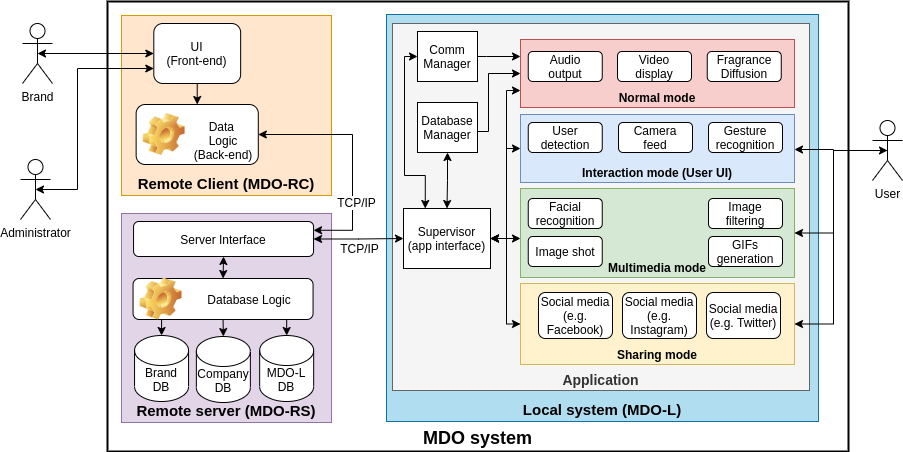
\includegraphics[width=1.0\columnwidth]{./img/sys-overview.png}
  \caption{\gls{mdo} system overview}%
\label{fig:sys-overview}
\end{figure}

Considering the system interactions, three main actors were identified:
\begin{enum-c}
\item \emph{Brand}: represents the brands contracting the advertisement
  services;
\item \emph{Administrator}: the development company staff, which can monitor and
  control the outdoor (administrative privileges).
\item \emph{User}: the user (the target audience of the advertisement)
  interacting with the system.
\end{enum-c}

Considering the data flow across the \textbf{MDO system}, three main subsystems were
identified: \textbf{\gls{mdo-rc}}, \textbf{\gls{mdo-rs}}, and
\textbf{\gls{mdo-l}}. The rational behind this initial decomposition is
explained next.

\subsection{MDO Remote Client}
The \emph{Brand} and \emph{Administrator} members require a remote \gls{ui} (front-end) to
interact with the system: the former to configure the advertisements being
displayed at the \gls{mdo} and purchase them; the latter to remotely monitor and
control the operation of the \gls{mdo}. Thus, it is clear that \emph{an
  authentication mechanism must be provided for the remote \gls{ui}}.

The data is then dispatched to the back-end, where it is processed and feed back
to the \gls{ui} user and/or sent to the remote server, via \gls{tcp-ip}
comprising the data logic component of the \gls{ui}.
%
%
\subsection{MDO Remote Server}
\label{sec:mdo-remote-server}
Although the \gls{mdo-rc} could communicate directly with the \gls{mdo-l}, this
is not desirable or a good architecture mainly due to: communications failure could
result in data loss, compromising the system's integrity; the remote client and
the local system become tightly coupled, meaning the remote client must be aware
of all the available local systems; if the data storage in the local system
fails, the remote client would have to provide the backup information.

Thus, a remote server component is included, providing the access and management
of the system databases, pertaining to the \emph{Brand}, \emph{Company}, and
\emph{MDO Local system}. The first two provide the historical information of the
\texttt{Brand} and \texttt{Administrator} entities, and the last one the information
related to all of the \texttt{\gls{mdo-l}} systems in operation.

The main functions of the \texttt{\gls{mdo-rs}} are:
\begin{item-c}
\item \emph{UI requests responses}: when a \gls{ui} user requests/modifies
  some information from the database, the server must provide/update it.
\item \emph{\gls{mdo-l} monitoring and control}: provide command dispatch and
  feedback to the \texttt{Administrator} staff for remote monitoring and control of
  the device.
\item \emph{\gls{mdo-l} update}: periodically check for start times of each
  \gls{mdo-l} device and transfer the relevant data to it.
\end{item-c}

The server interface is the responsible for managing the requests and respective
responses from the remote client and for periodically send the update data to
all \gls{mdo-l} devices. 
%
%
\subsection{MDO Local system}
\label{sec:mdo-local-system}
The \gls{mdo} local system (MDO-L) is the marketing device, interacting with the user
to display multi-sensory advertisements. As aforementioned in
Section~\ref{sec:prob-stat}, it is comprised of four modes:
\begin{item-c}
\item \emph{normal mode}: the MDO provides sound, video and fragrance
  outputs. It is the default mode.
\item \emph{interaction mode}: When a user approaches the device, the \gls{mdo} will
go into interaction mode, turning on and displaying the camera feed and waiting
for recognizable gestures to provide additional functionalities, such as
brand-specific image filters. This is the \texttt{User} \gls{ui}.
\item \emph{multimedia mode}: in this mode the facial recognition is applied,
  enabling the user to select and apply different brand-specific image filters and take pictures or create a \gls{gif}.
\item \emph{sharing mode}: after a user take a picture or create a \gls{gif}, it
  can share it across social media.
\end{item-c}

The user interaction is considered to be a higher priority activity than the
advertisements, so when a \texttt{User} interacts with the system, the \texttt{normal
mode} is overriden by the \texttt{Interaction mode}, thus, halting the
advertisements.

The \gls{mdo-l} application communicates with the remote server
(\texttt{\gls{mdo-rs}}) through the \texttt{Supervisor} via \gls{tcp-ip}
 to handle requests from \texttt{Administrator} members
to monitor and control the device through the \texttt{Supervisor} or to update
the advertisements. Additionally, the \texttt{Supervisor} oversees the
application mode and the communication (\texttt{Comm Manager}) and database
(\texttt{Database manager}) managers to handle system events.
%
%%% Local Variables:
%%% mode: latex
%%% TeX-master: "../../../dissertation"
%%% End:

% System Architecture
%
\section{System architecture}
\label{sec:system-architecture}
In this section, the system architecture is devised in the \gls{hw} and \gls{sw} components, using the system overview as a starting point. 

\subsection{Hardware architecture}
\label{sec:hardw-arch}
%
The diagram in Fig.\ref{fig:hw-arch} represents an initial hardware big picture in order to facilitate the objective identification.
As it can bee seen, the diagram is divided in four distinguished parts: \emph{External Environment}, \emph{Local System}, \emph{Remote Server} and \emph{Remote Client}.

Firstly, the \texttt{External Environment} represents all the environment that interacts with the system. In this case, these are all its users - normal users, brands and staff.

Secondly, the \texttt{Local System} is composed for the main controller, which is the Raspberry Pi 4B. 
This \gls{mcu} is responsible to controll all the Local System and to establish connection with the remote server through its included WiFi module. 
The board is powered connecting it to the electrical network. 
Then, it has several blocks connected to it:
%
\begin{item-c}
\item \emph{Motion Detection}: Used to detect the users and switch from normal mode to interaction mode;
\item \emph{Fragrance Diffusion Actuator}: used to diffuse the fragrance onto the air;
\item \emph{Camera}: Used to capture image that is then processed;
\item \emph{Speakers}: Used to produce advertisements sounds;
\item \emph{Screen}: Used to produce video clips of advertisements.
\end{item-c}
%

In third place, the \texttt{Remote Server} has a server node running in another machine that can be one computer or a main frame.
The remote server establishes connection with the cloud that has stored all the data from all databases.

Lastly, the \texttt{Remote Client} which can be a computer, a tablet or a smart phone to run the \gls{mdo} management application.
%
\begin{figure}
\centering
    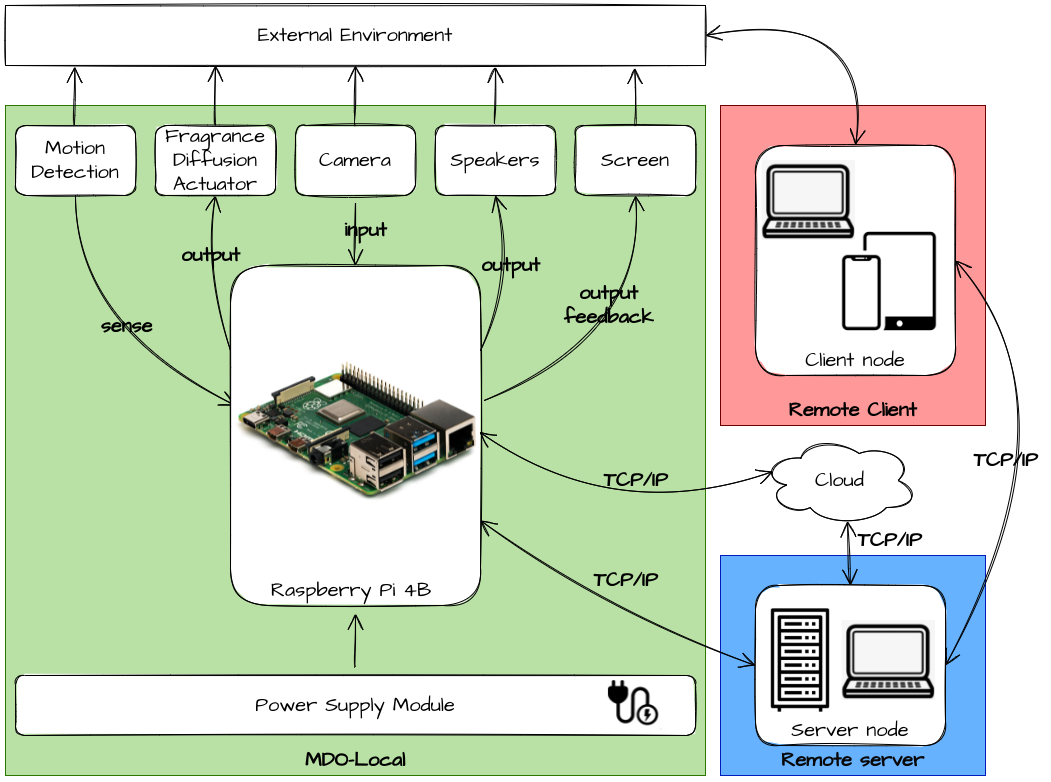
\includegraphics[width=0.9\columnwidth]{./img/HW_Architecture.png}
  \caption{~\gls{hw} Architecture Diagram}%
\label{fig:hw-arch}
\end{figure}
%
%
\subsection{Software architecture}
\label{sec:softw-arch}
In this section the \gls{sw} architecture for \gls{mdo-rc}, \gls{mdo-rs}, and
\gls{mdo-l} subsystems is presented, defining its \gls{sw} stack.

\subsubsection{MDO remote client}
\label{sec:mdo-remote-client}
Fig.~\ref{fig:sw-arch-rc} illustrates the \gls{sw} architecture for the remote
client, representing its \gls{sw} stack.
It is comprised of the following layers:
\begin{item-c}
\item \emph{Application}: contains the remote client application. The
  \texttt{Brand} and \texttt{Admin} members interact with the \gls{ui}, which is
  the visual part of the interface. The \texttt{\gls{ui} engine} is notified and
  handles all \gls{ui} events --- internal or external --- providing the \texttt{UI}
  with feedback for its users. The relevant commands
  are then parsed --- \texttt{Parser} component --- and responded. The commands
  are then translated to the appropriate \gls{db} queries and responded through
  the \texttt{DB Manager}. The \texttt{Comm Manager} is responsible for
  encapsulating the \gls{db} queries into the respective \gls{tcp-ip} frames to
  be sent to the \texttt{Remote Server} as well as unwrap the incoming server
  responses.
\item \emph{Middleware}: contains the \gls{tcp-ip} framework supporting these
  communication protocols as part of \gls{osi} model for internet
  applications. It manages the incoming/outgoing \gls{tcp-ip} frames by
  providing the adequate protocol handshaking and queueing and timing aspects of
  the bytes to send/receive.
\item \emph{OS \& BSP} --- \gls{os} \& \gls{bsp}: it contains the low-level and
  communication drivers required to handle input (keyboard/touch), output
  (screen) and communication to the \texttt{Remote Server}.
\end{item-c}
It should be noted that for desktop and mobile applications, the
\texttt{Middleware} and \texttt{OS \& BSP} layers are usually abstracted by the
\gls{os}, thus, the relevant \gls{api}s should be used.
%
\begin{figure}
\centering
    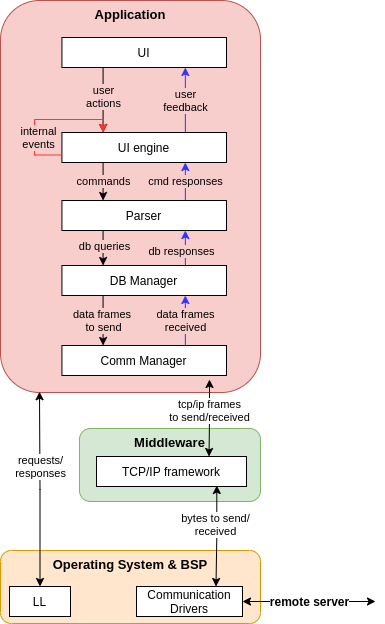
\includegraphics[width=0.55\columnwidth]{./img/sw-arch-rc.png}
  \caption{~\gls{sw} architecture diagram: remote client}%
\label{fig:sw-arch-rc}
\end{figure}

\subsubsection{MDO remote server}
\label{sec:mdo-remote-server-1}
%
Fig.~\ref{fig:sw-arch-rs} illustrates the \gls{sw} stack for architecture for
the remote server.
It is comprised of the following layers:
\begin{item-c}
\item \emph{Application}: contains the remote server application. It provides a
  \gls{cli} to handle \texttt{Remote client} requests.  The \gls{cli} engine
  is notified and handles all \gls{ui} events --- internal or external ---
  providing the appropriate feedback. The relevant commands
  are then parsed --- \texttt{Parser} component --- and responded: \gls{db}
  queries are handled by the \texttt{\gls{rdbms}} issuing \gls{db} transactions;
  other commands received by the \texttt{Remote Client} are handled internally
  and translated, being dispatched to the \texttt{Local
    System} by the \texttt{Comm Manager}  (via \texttt{Communication drivers}). Internal events can also
  trigger the \texttt{\gls{rdbms}} to issue database transactions for the
  \texttt{Remote Client} or \texttt{Local System}.
  The \texttt{Comm Manager} is responsible for wrapping\slash unwrapping the data
  frames received by or sent to the \texttt{Remote Client} or \texttt{Local System}.
\item \emph{Middleware}: contains the \gls{rdbms} framework supporting the
  management of the relational databases using database transactions.
\item \emph{OS \& BSP} --- \gls{os} \& \gls{bsp}: it contains the \texttt{Communication}
  drivers to the handle requests from the \texttt{Remote Client}, and the
  \texttt{File I/O} drivers to manipulate \gls{db} transactions from\slash to storage.
\end{item-c}
%
\begin{figure}
\centering
    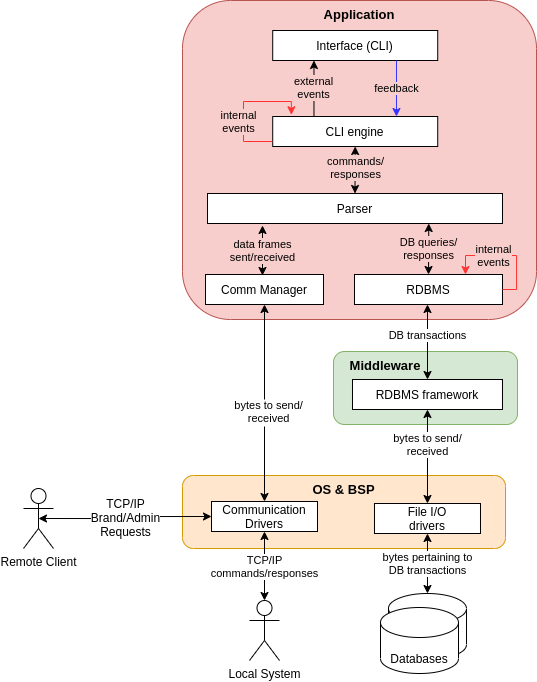
\includegraphics[width=0.55\columnwidth]{./img/sw-arch-rs.png}
  \caption{~\gls{sw} architecture diagram: remote server}%
\label{fig:sw-arch-rs}
\end{figure}
%
\subsubsection{MDO local system}
\label{sec:mdo-local-system-1}




%%% Local Variables:
%%% mode: latex
%%% TeX-master: "../../../dissertation"
%%% End:

% Subsystem decomposition

\section{Subsystem decomposition}
\label{sec:subsyst-decomp}

For each subsystem, do:
1. Events
2. Use cases
3. State machine diagram
4. Sequence diagram

\subsection{Local system}
\label{sec:local-system}

\subsubsection{Events}
\label{sec:events}

\subsubsection{Use cases}
\label{sec:use-cases}

\subsubsection{Dynamic operation}
\label{sec:dyn-oper}
State machine diagram

\subsubsection{Flow of events}
\label{sec:flow-events}
Sequence diagram

\subsection{Remote system}
\label{sec:remote-system}

\subsubsection{Events}
\label{sec:events-1}

\subsubsection{Use cases}
\label{sec:use-cases-1}

\subsubsection{Dynamic operation}
\label{sec:dyn-oper-1}
State machine diagram

\subsubsection{Flow of events}
\label{sec:flow-events-1}
Sequence diagram


%%% Local Variables:
%%% mode: latex
%%% TeX-master: "../../../dissertation"
%%% End:

% Budget estimation
%
\section{Budget estimation}
\label{sec:budget-estimation}
% Please add the following required packages to your document preamble:
% \usepackage{booktabs}
% \usepackage{multirow}
% \usepackage[table,xcdraw]{xcolor}

\begingroup
\renewcommand{\arraystretch}{1.1} % Default value: 1
\begin{table}[!hbt]
\addtolength{\tabcolsep}{-2pt}
\footnotesize
\centering
\caption{Budget estimation}
\label{tab:budget-estimation}
\begin{tabular}{llrlr}
\hline
                                                                                                                   & \multicolumn{2}{c}{\textbf{Scale-model Prototype}}                            & \multicolumn{2}{c}{\textbf{Real-scale Prototype}}                                                       \\ \hline
                                                                                                                   & \textbf{Item}                       & \multicolumn{1}{l}{\textbf{Cost (€) *}} & \textbf{Item}                                                 & \multicolumn{1}{l}{\textbf{Cost (€) *}} \\ \hline
\rowcolor[HTML]{FFCE93} 
\cellcolor[HTML]{FFCE93}                                                                                           & Raspberry Pi 4B                     & 50                                      & \cellcolor[HTML]{FFDBB0}Raspberry Pi 4B                       & \cellcolor[HTML]{FFDBB0}50              \\ \cline{2-5} 
\rowcolor[HTML]{FFCE93} 
\cellcolor[HTML]{FFCE93}                                                                                           & User Detection sensor               & 3                                       & \cellcolor[HTML]{FFDBB0}User Detection sensor mesh (4)        & \cellcolor[HTML]{FFDBB0}12              \\ \cline{2-5} 
\rowcolor[HTML]{FFCE93} 
\cellcolor[HTML]{FFCE93}                                                                                           & LCD display 10” (non-touch)         & 55                                      & \cellcolor[HTML]{FFDBB0}LCD display 55” Full HD (non-touch)   & \cellcolor[HTML]{FFDBB0}1500            \\ \cline{2-5} 
\rowcolor[HTML]{FFCE93} 
\cellcolor[HTML]{FFCE93}                                                                                           & Fragrance diffusion actuator        & 5                                       & \cellcolor[HTML]{FFDBB0}Fragrance diffusion actuator mesh (4) & \cellcolor[HTML]{FFDBB0}20              \\ \cline{2-5} 
\rowcolor[HTML]{FFCE93} 
\cellcolor[HTML]{FFCE93}                                                                                           & Camera 8 MP                         & 32                                      & \cellcolor[HTML]{FFDBB0}Camera 8 MP                           & \cellcolor[HTML]{FFDBB0}32              \\ \cline{2-5} 
\rowcolor[HTML]{FFCE93} 
\cellcolor[HTML]{FFCE93}                                                                                           & Speakers                            & 5                                       & \cellcolor[HTML]{FFDBB0}Speakers                              & \cellcolor[HTML]{FFDBB0}30              \\ \cline{2-5} 
\rowcolor[HTML]{FFCE93} 
\cellcolor[HTML]{FFCE93}                                                                                           & Power supply                        & 10                                      & \cellcolor[HTML]{FFDBB0}Power supply                          & \cellcolor[HTML]{FFDBB0}30              \\ \cline{2-5} 
\rowcolor[HTML]{FFCE93} 
\multirow{-8}{*}{\cellcolor[HTML]{FFCE93}\textbf{HW}}                                                              & PCB                                 & 8                                       & \cellcolor[HTML]{FFDBB0}PCB                                   & \cellcolor[HTML]{FFDBB0}16              \\ \hline
\rowcolor[HTML]{FFCE93} 
\cellcolor[HTML]{FFCE93}                                                                                           & 3D printed + screws                 & 20                                      & \cellcolor[HTML]{FFDBB0}Built-in with display + HW packaging  & \cellcolor[HTML]{FFDBB0}100             \\ \cline{2-5} 
\rowcolor[HTML]{FFCE93} 
\multirow{-2}{*}{\cellcolor[HTML]{FFCE93}\textbf{\begin{tabular}[c]{@{}l@{}}Mechanical \\ Structure\end{tabular}}} &                                     &                                         & \cellcolor[HTML]{FFDBB0}Full HW packaging                     & \cellcolor[HTML]{FFDBB0}350             \\ \hline
\rowcolor[HTML]{FFCE93} 
                                                                                                                   & \textbf{Physical Prototype cost}    & \textbf{188}                            & \cellcolor[HTML]{FFDBB0}\textbf{Physical Prototype cost **}   & \cellcolor[HTML]{FFDBB0}\textbf{2040}   \\ \hline
\rowcolor[HTML]{FFFE8A} 
\cellcolor[HTML]{FFFE8A}                                                                                           & Remote Client: 500 h ***            & 5000                                    & \cellcolor[HTML]{FFFFC7}Remote Client: 500 h ***              & \cellcolor[HTML]{FFFFC7}5000            \\ \cline{2-5} 
\rowcolor[HTML]{FFFE8A} 
\cellcolor[HTML]{FFFE8A}                                                                                           & Remote Server: 300 h ***            & 3000                                    & \cellcolor[HTML]{FFFFC7}Remote Server: 300 h ***              & \cellcolor[HTML]{FFFFC7}3000            \\ \cline{2-5} 
\rowcolor[HTML]{FFFE8A} 
\multirow{-3}{*}{\cellcolor[HTML]{FFFE8A}\textbf{\begin{tabular}[c]{@{}l@{}}SW \\ development\end{tabular}}}       & Local system: 1000 h ***            & 10000                                   & \cellcolor[HTML]{FFFFC7}Local system: 1000 h ***              & \cellcolor[HTML]{FFFFC7}10000           \\ \hline
\rowcolor[HTML]{FFFE8A} 
                                                                                                                   & \textbf{SW development cost}        & \textbf{18000}                          & \cellcolor[HTML]{FFFFC7}\textbf{SW development cost}          & \cellcolor[HTML]{FFFFC7}\textbf{18000}  \\ \hline
\rowcolor[HTML]{D5FBFC} 
\cellcolor[HTML]{D5FBFC}                                                                                           & Local System power consumption **** & 0                                       & \cellcolor[HTML]{E2FEFF}Local System power consumption ****   & \cellcolor[HTML]{E2FEFF}0               \\ \cline{2-5} 
\rowcolor[HTML]{D5FBFC} 
\multirow{-2}{*}{\cellcolor[HTML]{D5FBFC}\textbf{\begin{tabular}[c]{@{}l@{}}Operational \\ costs\end{tabular}}}    & Server operation cost *****         & 420                                     & \cellcolor[HTML]{E2FEFF}Server operation cost *****           & \cellcolor[HTML]{E2FEFF}420             \\ \hline
\rowcolor[HTML]{D5FBFC} 
                                                                                                                   & \textbf{Yearly Operational cost}    & \textbf{420}                            & \cellcolor[HTML]{E2FEFF}\textbf{Yearly Operational cost}      & \cellcolor[HTML]{E2FEFF}\textbf{420}    \\ \cline{2-5} 
                                                                                                                   & \textbf{Total cost}                 & \textbf{18608}                          & \textbf{Total cost}                                           & \textbf{20460}                          \\ \cline{2-5} 
\multicolumn{2}{l}{* tax included}                                                                                                                       & \multicolumn{1}{l}{}                    &                                                               & \multicolumn{1}{l}{}                    \\
\multicolumn{2}{l}{** considering the most expensive option}                                                                                             & \multicolumn{1}{l}{}                    &                                                               & \multicolumn{1}{l}{}                    \\
\multicolumn{2}{l}{*** 10 €/h}                                                                                                                           & \multicolumn{1}{l}{}                    &                                                               & \multicolumn{1}{l}{}                    \\
\multicolumn{2}{l}{**** 24h/7d for 1 year}                                                                                                               & \multicolumn{1}{l}{}                    &                                                               & \multicolumn{1}{l}{}                    \\
\multicolumn{2}{l}{***** yearly cost}                                                                                                                    & \multicolumn{1}{l}{}                    &                                                               & \multicolumn{1}{l}{}                    \\ \hline
\end{tabular}
\end{table}
\endgroup
% 
%%% Local Variables:
%%% mode: latex
%%% TeX-master: "../../../dissertation"
%%% End:

% \section{Project planning}
\label{sec:project-planning}

\subsection{Budget}
\label{sec:budget}


%%% Local Variables:
%%% mode: latex
%%% TeX-master: "../../../dissertation"
%%% End:

% Theoretical foundations
% \subsection{Waterfall}%
\label{subsec:waterfall}
For the domain-specific design of software the waterfall methodology is used.
The waterfall model (fig.~\ref{fig:waterfall}) represents the first effort to
conveniently tackle the increasing complexity in the software development
process, being credited to Royce, in 1970, the first formal description of the
model, even though he did not coin the term~\cite{sommerville1996software}. It
envisions the optimal method
as a linear sequence of phases, starting from requirement elicitation to system
testing and product shipment~\cite{cusumano1995beyond} with the process flowing
from the top to the bottom, like a cascading waterfall.

In general, the phase sequence is as follows: analysis, design, implementation,
verification and maintenance.
\begin{enumerate}
  \item Firstly, the project requirements are elicited, identifying the key
    requirements and constraints the system being developed must meet from the
    end-user perspective, captured in natural language in a product requirements document.
  \item In the analysis phase, the developer should convert the application
    level knowledge, enlisted as requirements, to the solution domain knowledge
    resulting in analysis models, schema and business rules.
  \item In the design phase, a thorough specification is written allowing the
    transition to the implementation phase, yielding the decomposition in
    subsystems and the software architecture of the system. 
  \item In the implementation stage, the system is developed, following the
    specification, resulting in the source code.
  \item Next, after system assembly and integration, a verification phase occurs
    and system tests are performed, with the systematic discovery and debugging
    of defects.
  \item Lastly, the system becomes a product and, after deployment, the
    maintenance phase start, during the product life time.
\end{enumerate}
While this cycle occurs, several transitions between multiple phases might
happen, since an incomplete specification or new knowledge about the system,
might result in the need to rethink the document.

The advantages of the waterfall model are: it is simple and easy to understand
and use and the phases do not overlap; they are completed sequentially. However,
it presents some drawbacks namely: difficulty to tackle change and high
complexity and the high amounts of risk and uncertainty. However, in the present
work, due to its simplicity, the waterfall model proves its usefulness and will
be used along the project.

As a reference in the sequence of phases and the expected outcomes from each
one, it will be used the chain of development activities and their products
depicted in fig.~\ref{fig:sw-devel-activities} (withdrawn from
\cite{bruegge2004object}).

\begin{figure}[!hbt]
\centering
    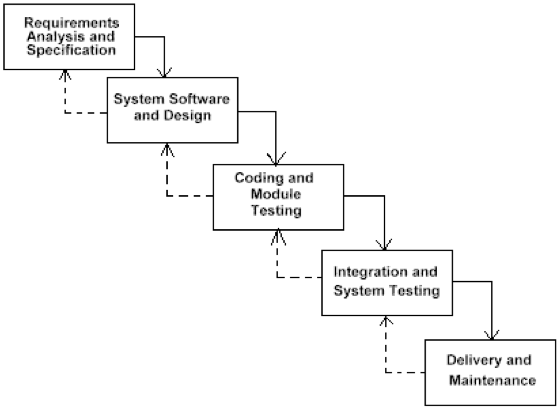
\includegraphics[width=0.6\textwidth]{./img/waterfall.png}
  \caption{Waterfall model diagram}\label{fig:waterfall}
\end{figure}

\subsection{Unified Modeling Language (UML)}
\label{subsec:uml}
To aid the software development process, a notation is required, to articulate
complex ideas succinctly and precisely. The notation chosen was the \gls{uml},
as it provides a spectrum of notations for representing different aspects of a
system and has been accepted as a standard notation in the software
industry~\cite{bruegge2004object}.

The goal of UML is to provide a standard notation that can be used by all
object- oriented methods and to select and integrate the best elements of
precursor software notations, namely \gls{omt}, Booch, and \gls{oose}
~\cite{bruegge2004object}. It provides
constructs for a broad range of systems and activities (e.g., distributed
systems, analysis, system design, deployment). System development focuses on
three different models of the system
(fig.~\ref{fig:sw-devel-activities})~\cite{bruegge2004object}:
\begin{enumerate}
  \item \textbf{\emph{The functional model}}: represented in UML with use case
    diagrams, describes the functionality of the system from the user's point of
    view.
  \item \textbf{\emph{The object model}}: represented in UML with class
    diagrams, describes the structure of the system in terms of objects,
    attributes, associations, and operations.  
  \item \textbf{\emph{The dynamic model}}: represented in UML with interaction
    diagrams, state-machine diagrams, and activity diagrams, describes the
    internal behaviour of the system.
\end{enumerate}

\begin{figure}[!hbt]
\centering
    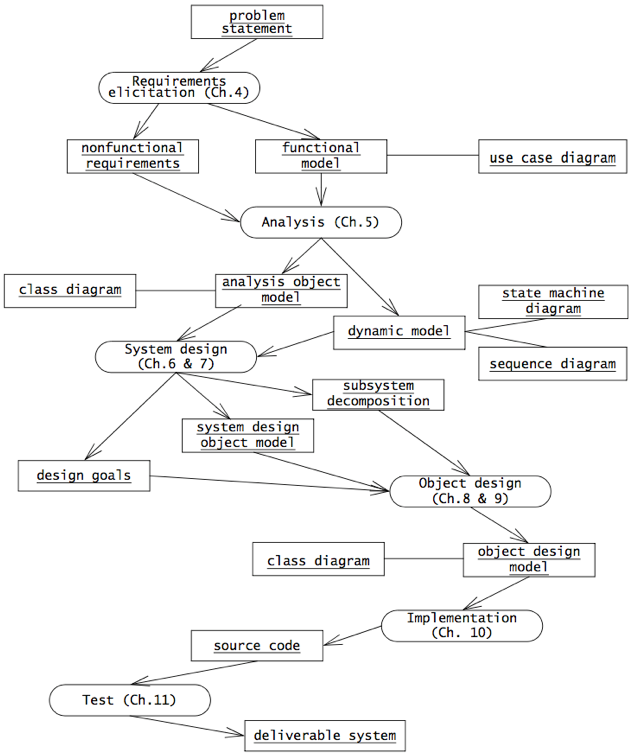
\includegraphics[width=0.7\textwidth]{./img/sw-devel-activities.png}
  \caption{An overview of the object-oriented software engineering development
  and their products. This diagram depicts only logical dependencies among work
  products (withdrawn from~\cite{bruegge2004object})}
\label{fig:sw-devel-activities}
\end{figure}
%%% Local Variables:
%%% mode: latex
%%% TeX-master: "../../../dissertation"
%%% End:

%
%%% Local Variables:
%%% mode: latex
%%% TeX-master: "../../../dissertation"
%%% End:

\setcounter{table}{0}
\setcounter{figure}{0}
%
\chapter{Design}
\label{ch:design}
In this section the theoretical foundations are used to design a viable
solution, accordingly to the requirements and constraints listed.
In the design phase, the product development starts, specifying the system in
terms of hardware and software and its associated interfaces, the error handling
required, and the design verification.
%
  \vspace{-5mm}
%  
\section{Hardware specification}
\label{sec:hw-specs}
The first step for system design is the \gls{hw} specification. This can be
pictured as a block diagram, ideally with \gls{cots}
components. Fig.~\ref{fig:block-diag} depicts the overall information flow and
the TV remote block diagram: the \texttt{User} interacts with
the TV remote by pressing buttons which triggers the emission of \gls{ir} codes
to the TV, containing the \gls{ir} receiver. As supported by the market research
seen in
Section~\ref{sec:market-research}, the block diagram of the TV remote control
can be taught of a physical input interface --- the pushbuttons, a processing
interface --- a microprocessor --- to determine which keys are pressed and the
resulting \gls{ir} codes to be emitted, and a \gls{ir} transmitter circuit as
the output where the IR LED also works as a visual output. Usually, there will
be also a digital interface, to handle the large amount of keys as a
\gls{io} expander with serial interface, e.g. the Microchip MCP23008/MCP23S08~\cite{microchip}, which is considered here for future expansibility of the device,
thus making it scalable. This can be especially useful when using
microprocessor units with lower I/O inputs. A tradeoff between the inclusion of
the multiplexer versus future redesign must be performed.

The microprocessor chosen depends on various factors, such as: architecture,
throughput, memory, processing power, power efficiency, toolchain availability
and programming easiness, etc. Additionally, one may consider the usage of a
microcontroller, due to added peripherals, easing the \gls{sw} burden. For
example, the usage of the \gls{pca} peripheral in the 8051 \gls{mcu} can free the processor from the
job of bit-banging the IR transmitter circuitry or the \gls{i2c} or \gls{spi} peripherals to
interface the I/O expander. With that said, the choice
relied on the 8051 MCU due to its small footprint, clock speed of up to 48 MHz,
low power usage on idle, the acquaintance with the toolchain and the
programming, and for the inclusion of the PCA, SPI and I2C peripherals.  
%
  \vspace{-5mm}
%  
%- Block diagram with COTS components, if possible
%- List of constraints of functions to be implemented in HW or SW
%  - Inclusion of a multiplexer may reduce SW burden
%  - CPU peripherals:
%  - PCA for wave generation
%  
\begin{figure}[htb!]
\centering
    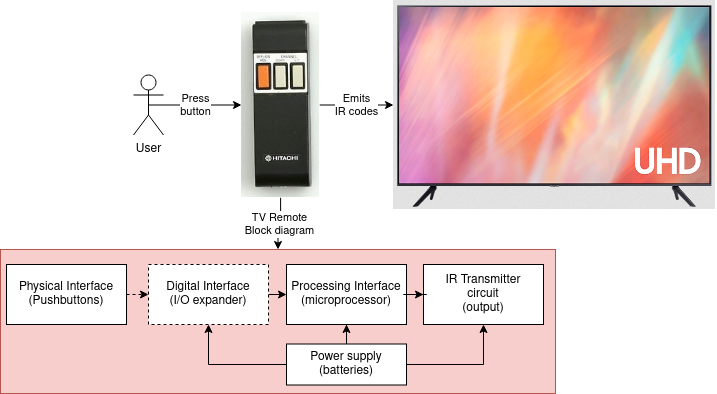
\includegraphics[width=0.7\columnwidth]{./img/block-diagram.png}
  \caption{Overall information flow and TV remote block diagram}%
\label{fig:block-diag}
\end{figure}
%
  \vspace{-5mm}
%  
\section{Hardware interfaces definition}
\label{sec:hw-interf-def}
After specifying the \gls{hw}, it is important to define its interfaces. The
TV remote control is clearly an event-driven asynchronous system, thus using HW
interrupts. When a user presses a pushbutton that event should be signaled to
the \gls{cpu} of the MCU via an external interrupt, ``waking'' it up. The CPU
handles that interrupt via an \gls{isr}, processing it and actuating, if
required. The system then goes back to sleep.

The 8051 MCU only contains 2 external interrupts sources --- \texttt{EXT0} and
\texttt{EXT1} --- thus limitting the direct connection of the pushbuttons to the
MCU, even with the pull-up circuitry. This is where the serial I/O expander
becomes most useful, as it can be connected to TV remote keys (up to 8 in this
case) and connected to a single external interrupt pin, being then read via
\gls{i2c} or \gls{spi} interface. Thus, the keys can be connected through
pull-up circuitry to the I/O expander and the output is then connected to
\texttt{EXT0} on the 8051 MCU. The communication protocol chosen is \gls{i2c} as
it is more expandable

Concerning the output, the 8051 PCA peripheral is connected to the IR
transmitter circuitry, for IR code emission.
%
  \vspace{-5mm}
%  
\section{Software specification}
\label{sec:sw-specs}
Top-down methodology
1. Identify main subsystems
   1. Signal input detector
   2. Event handler
   3. Output generator
%
  \vspace{-5mm}
%  
\section{Software interfaces definition}
\label{sec:sw-interf-def}
- Define the APIs in detail:
  - header files with:
    - functions prototypes
    - data structure declarations
    - class declarations

\section{Start-up/shutdown process specification}
\label{sec:startup-shutdown}
%
  \vspace{-5mm}
%  
\section{Error handling specification}
\label{sec:error-handling-specification}
- Create error-handling routines
- Watchdog timer can be used for system recovery
%
  \vspace{-5mm}
%  
\section{Design verification}
\label{sec:design-verification}
%
  \vspace{-5mm}
%  
%%% Local Variables:
%%% mode: latex
%%% TeX-master: "../../dissertation"
%%% End:

\setcounter{table}{0}
\setcounter{figure}{0}

%  	% CHAPTER - Conclusion/Future Work --------------
\chapter{Conclusion}%
\label{ch:conclusion}
In this chapter are outlined the conclusions and the prospect for future work
regarding the autonomous navigation of robots.
%
\section{Conclusions}%
\label{ch:conclusion-concls}
The Marketing Digital Outdoor can be described as a system was developed to help brands to share their products in a more efficient and attractive way through a photo booth with gesture recognition and face based filters, video and sound display, pictures and gif taking and also fragrance emission.

The analysis was well thought since the first moments. A development of a distributed architecture was obviously the most expandable and efficient way to solve the problem statement.

The implementation phase brings another robustness and consolidation to the analysis with something more deep 

The autonomous navigation of robots can be described as a collision-free path
towards a target and successfully formulated and implemented using dynamic
systems. Amongst the class of the dynamic systems, the nonlinear type arises as
the most useful due to variations of qualitative behavior --- number and or/or
stability of the fixed points of the dynamic system. 

Then, the behaviors were analyzed in isolation and in integration, namely target
acquisition and obstacle avoidance, strongly supported by a previous analytical
study of the corresponding dynamic system. This analytical study, based on the
qualitative theory of dynamic systems, consisted in the determination of the
fixed points and its stability, the corresponding phase portraits, i.e.,
possible evolution of the system's state, and the bifurcation diagram, yielding
the bifurcation points as a function of the parameters of the system.
\\\\
\textbf{Target Acquisition}: An autonomous mobile robot must be able to navigate to a target position. The
target acquisition behavior can be yielded by dynamic systems for the heading
direction and path velocity (Eq.~(\ref{eq:3}) and Eq.~(\ref{eq:4})). The heading direction dynamics consists of a
sinusoidal function (Eq.~(\ref{eq:5})), as it is required the heading direction
converges to the target independently of its initial state, yielding an attractor in the heading direction and a
repeller in the opposite one for faster convergence. 

The implementation of the
dynamic systems was performed using Forward Euler's method in Matlab, and used
to command a simulation in CoppeliaSim environment. Several scenarios were
simulated for different velocities functions, and was observed that a dynamic
system for path velocity is required for adequate velocity control. Alongside
with these simulations, the system's parameters were tuned, namely the time
constants of the system. 

Lastly, a linear dynamic system for heading direction
was considered and compared to the nonlinear one. 
It was observed the nonlinear
dynamic system is better suited for the target acquisition behavior of the
robot, as it provides smoother paths --- narrower angular velocity range.
\\\\
\textbf{Obstacle avoidance}: While moving to a target, a robot must also avoid obstacles that may appear ---
obstacle avoidance. To avoid obstacles, the robot must firstly detect them, in
this case, using infrared radiation sensors. The strategy adopted consisted in
assuming that each sensor $i$ specifies a virtual obstacle in the direction
$\psi_{obs,i}$ if an obstruction is detected in that direction, modelled by a
repulsive force centered in the direction the respective sensor points out,
$f_{obs,i}$ (Eq.~(\ref{eq:24})). As each sensor is mounted in a fixed direction
$\theta_i$ in respect to the frontal direction of the robot, the calibration of
the system is unnecessary. 

The obstacle avoidance dynamics establishes a
repeller in the virtual obstacle direction with variable strength, as a function
of the distance to obstacles (Eq.~(\ref{eq:25})) --- high for small distances
and low for high distances --- and where the angular range over which the
force-let exerts its repulsive effect should be limited
(Eq.~(\ref{eq:26})). Gaussian white noise is also added to the dynamics to
enable the escape from the repeller in a finite time, in case this is the
initial condition. 

The implementation was performed in Matlab using Forward
Euler's method. Several simulations were then performed to evaluate the impact
of parameters' variations, namely the maximum strenght of repulsion,
$\beta_1$, the decay rate of the repulsion force with the distance increase,
$\beta_2$, and noise magnitude $Q$. $\beta_1$ relates to the minimum time
constant of the obstacle avoidance dynamics $\tau_{obs,i}$ (Eq.~(\ref{eq:32})),
and for the simulations performed $\beta_1 = 3.5 \Delta t$. It should be noted,
however, that the value of this parameter is dependent on the rate of fixed
points shift. As for the parameter $\beta_2$, for increasing values the decay
rate diminishes, maintaining the repulsive effect significantly for
a wider distance range --- the robot starts to rotate farther away from the
obstacles. Conversely, for decreasing values of $\beta_2$, the decay rate
increases, maintaining the repulsive effect significantly for
a narrow distance range --- the robot starts to rotate closer to the
obstacles. The addition of noise is important, but should be limited in
magnitude to avoid jitter: it should be sufficient enough to guarantee the escape from the
repellers within a time limit, in case the system is initially placed
there. Additionally, noise induces different qualitative behaviors (turn
left/right) due to stochastic effect. It was also noted that noise may not
always be required, as the system may present slight bias in sensors
readings. 

The simulations with different gap between obstacles showed a
the heading direction dynamics
exhibits different qualitative behaviors --- the stability of the fixed
points varies --- starting from gap = 50 cm. This corresponds to a bifurcation
point, representing the distance below which the robot
(with diameter 45 cm) cannot pass between the two obstacles. For gap < 50 cm, the planning dynamics has an reppeller
at the heading direction $\phi = \pi/2$, and for gap > 50 this reppeller becomes
asymptotically stable (i.e., an attractor). 

Lastly, a simulation was performed
in an environment with multiple obstacles, with the robot successfully and
adequately avoiding all of them.
\\\\
\textbf{Integration: Obstacle avoidance and Target acquisition}:
Next, the obstacle avoidance and target acquisition behaviors were integrated,
considering two approaches for the latter: nonlinear or linear dynamic
system. For both approaches the obstacle avoidance behavior must take precedence over the target acquisition
to prevent the robot from hitting an obstacle while attempting to move to the
target. This is guaranteed by imposing greater magnitude for repulsive component than for
attractive one, i.e. $\lambda_{obs} \gg \lambda_{tar}$, and consequently,
$\tau_{obs} \ll \tau_{tar}$.
After analyzing the robot's behavior for both nonlinear and linear dynamics, it
is was possible to compare them.
Mathematically, the fact that the nonlinear function is a sinusoidal function, yielding always
two fixed points --- one attractor, and in the opposite direction a
repeller --- whereas the linear function only contributes with one attractor to
the vector field. 
The repeller in the opposite direction to the target reinforces the heading direction that must be taken by the robot so that it reaches the target.
In the previous experiments, as well by Section~\ref{sec:discussion-linear-phi},
it is concluded by experimentation too, that the nonlinear system provides smoother paths at narrower angular velocity range.
Thus, it can be concluded that the nonlinear dynamic system is better for the target acquisition behavior of the robot. 
%
\\\\
\textbf{Control of driving speed}
The stability of the planning dynamics is affected by the rate of fixed points
shift, as to keep the system stable, i.e. in or near an attractor at all times, the rate of such
shifts must be limited to permit the track the attractor as it shifts. One way
of accomplishing this is by controlling the path velocity of the vehicle, as the
rate of fixed points shift is determined by the relative velocity of the robot
with respect to its environment~\cite{bicho2000dynamic}.

The shifting of fixed points for the planning dynamics can stem from robot
movement through the environment and associated sensory information 
changes or due to environmental changes (obstacles moving in the world), causing
attractors and repellers to change. 

Thus, a more adequate dynamic system for path velocity was
established, as the sum of obstacles and target contributions, where one of the
components dominates at all times. A systematic way to construct a
function that indicates if obstacles contributions are present, is to integrate
force-lets, from which a potential function of the obstacle avoidance dynamics
results. If the potential is positive a repeller is established for the planning
dynamics, and conversely, if negative an attractor arises. A convenient way 
to transform the potential levels to the strengths of the two contributions
to the velocity control is through the use of a sigmoidal threshold function,
defining the angular range the obstacles contribution is noticeable.

Then, the parameters were tuned considering the hierarchy of relaxation rates
--- which ensures that the system relaxes to the attractors and that obstacle
avoidance has precedence over the target --- and some rules of thumb for the
remaining path velocity parameters.

Finally, two scenarios were simulated --- S and Tar-Obs --- to assess the
performance of the overall dynamics. It was shown that, although the average
velocity was increased, the planning dynamics remains robust, suggesting a performance improvement in the overall dynamics.
%
\\\\
\textbf{Final remarks}:
Dynamic systems can be used to successfully implement the autonomous mobile
navigation of robots in a robust way, as the system follows closely the
asymptotically stable states, i.e. the attractors, yielding it robust to noise
and external disturbances. Specifically, nonlinear dynamic systems provide a
richness of qualitative behaviors as required for the highly dynamic conditions
imposed by the surroundings. Although more complex than the linear counterparts,
the qualitative theory of dynamic systems provides a convenient framework for a
relatively easy analysis of nonlinear dynamic systems.

The autonomous navigation of robots can be described as a collision-free path
towards a target, thus requiring both obstacle avoidance and target acquisition
behaviors for the planning dynamics. For the former, a repeller is established in the direction of the
virtual obstacles detected by the robot's sensor; for the latter, an attractor
is established in the direction of the target and a repeller in the opposite
direction for faster convergence of the desired heading direction. In the
integration of both behaviors the hierarchy of time constants must be observed,
assuring obstacle avoidance precedence over target acquisition and in a adequate
form, related to the computing time of the system.

To keep the planning dynamics stable, i.e. in or near an attractor at all times, the rate of such
shifts must be limited to permit the track the attractor as it shifts. One way
of accomplishing this is by controlling the path velocity of the vehicle, as the
rate of fixed points shift is determined by the relative velocity of the robot
with respect to its environment~\cite{bicho2000dynamic}. Thus, a more adequate
dynamic system for path velocity can be established using obstacles and target
contributions to the dynamic through a thresholded potential function and a
convenient tuning of the system.
%
\section{Prospect for Future Work}%
\label{ch:conclusion-future-work}
In the foreseeable future, the deployment of the planning and path velocity
dynamics to hardware could be performed, analyzing the navigation behavior of
the robot in real world scenarios. Additionally, the detection of targets could
be performed by the robot using different techniques such as sound detection or
computer vision.

Another interesting feature is to incorporate artificial intelligence to the
robot, enabling it to recall the most relevant target and to forget the others,
making it even more adaptable to the highly dynamic conditions of the surroundings. 
%%% Local Variables:
%%% mode: latex
%%% TeX-master: "../../dissertation"
%%% End:

%  \setcounter{table}{0}
%  \setcounter{figure}{0}
  % -----------------------------------------------------------------
  %
	\bookmarksetup{startatroot} % Ends last part.
	%\addtocontents{toc}{\bigskip} % Making the table of contents look good.
	%\cleardoublepage
%
	%- Bibliography (needs bibtex) -%
  % Using relative paths: 
  % src: https://tex.stackexchange.com/questions/38287/creating-a-central-bibliography
  %\addcontentsline{toc}{chapter}{Bibliography}
  \bibliography{./bib/dissert}
%
  % bibliography - tutorial: 
  % https://en.wikibooks.org/wiki/LaTeX/Modular_Documents
  %\clearpage %see what this means
  %\include{./tex/mybibliography}
%
  % ---------------------- APPENDIX ------------------------------------
  % renew figures and tables to use Alphabetic numbering and set counter to zero
  % src: https://tex.stackexchange.com/questions/118606/numbering-tables-a1-a2-etc-in-latex#comment862599_311998
%%  \setcounter{table}{0}
%%  \setcounter{figure}{0}
%%  \renewcommand{\thetable}{\Alph{chapter}.\arabic{table}}  
%%  \renewcommand{\thefigure}{\Alph{chapter}.\arabic{figure}}
%% %
%%  % Adding a page to separate appendices from the other chapters
%%  \chapter*{Appendices}%
%%\label{ch:Append}
%%  \addcontentsline{toc}{chapter}{\normalfont\scshape{Appendices}}
%%  \cleardoublepage%
%%%
%%  %\appendix % this is the normal appendix; we use a custom one
%%  \umappendix{Appendix}
%
  % Appendix chapters inclusion
%  % APPENDICES.tex: contains all appendices used
\setcounter{table}{0}
\setcounter{figure}{0}
% the appendix no longer requires the prefix Appendix <Letter>
\chapter{Project Planning --- Gantt diagram}%
\label{ch:append-gantt-diag}
In Fig.~\ref{fig:gantt-diag-orig} is illustrated the Gantt chart for the
project, containing the tasks' descriptions.
%%%%%%%%%%%%%%% Figure is deprecated: use PDF instead
%\begin{figure}[!htbp]
%\centering
%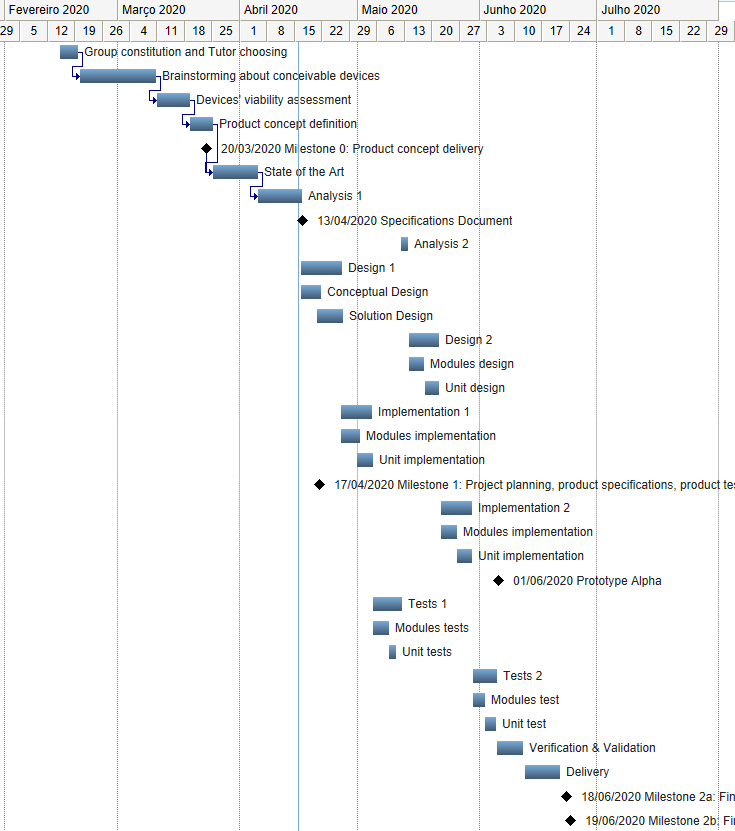
\includegraphics[width=1.0\textwidth]{./sec/img/gantt-diag-orig.png}
%\caption{\label{fig:gantt-diag2}Project planning: Gantt diagram 1}
%\end{figure}
%\begin{figure}[!htbp]
%\centering
%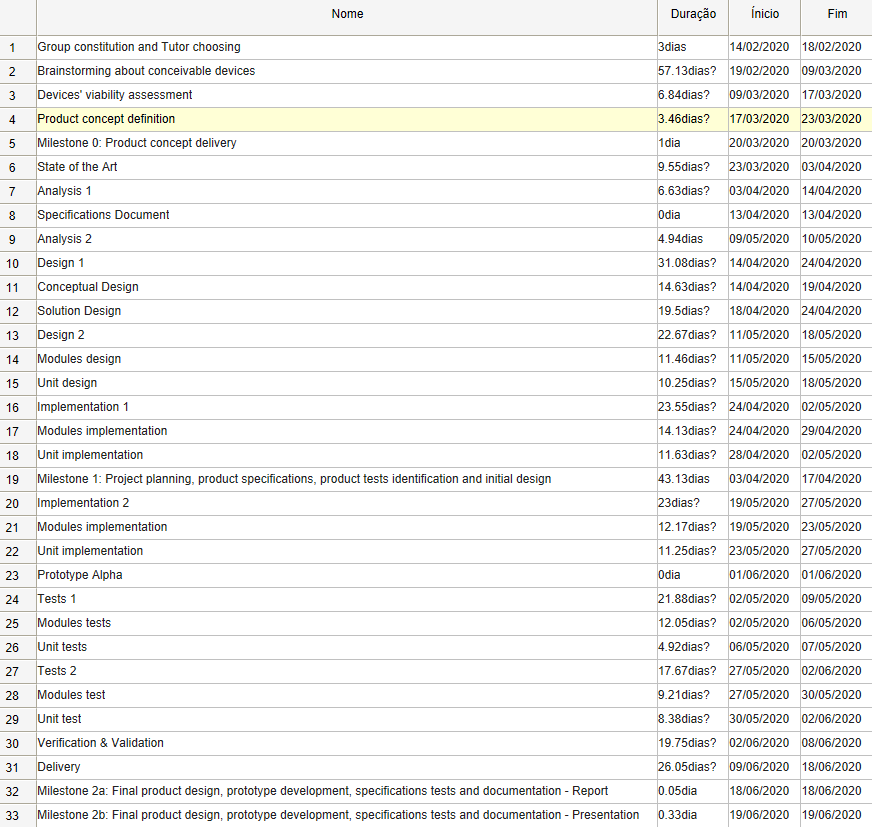
\includegraphics[width=1.0\textwidth]{./sec/img/gantt-orig-tasks.png}
%\caption{\label{fig:gantt-tasks}Project planning: tasks}
% \end{figure}
%%%%%%%%%%%%%%%%%%%%%%%%%%%%%%%%%%%%%%%%%%%%%%%%%%%%%%%%%%%%%
% 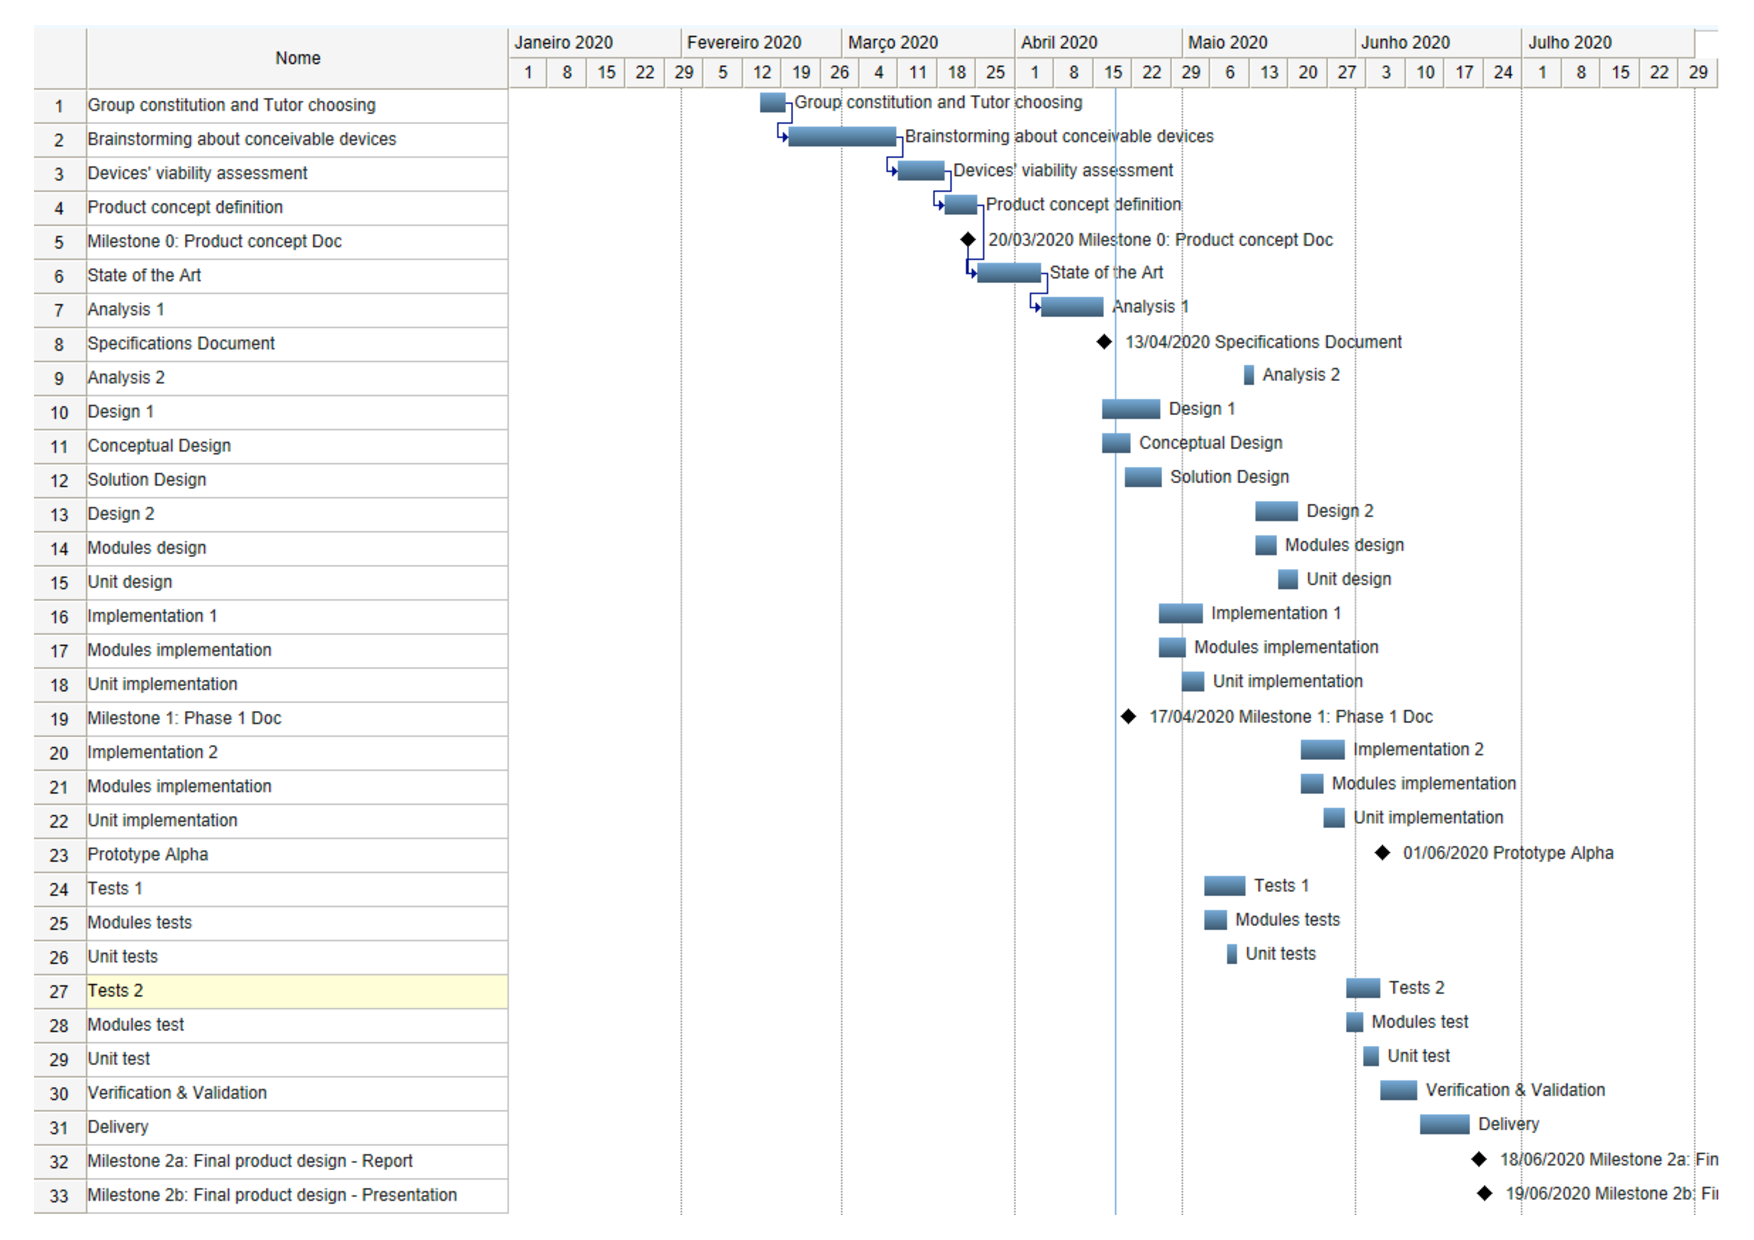
\includepdf[pages=-]{sec/pdf/gantt-diag-orig.pdf}
\begin{sidewaysfigure}[!h]
  \centering
  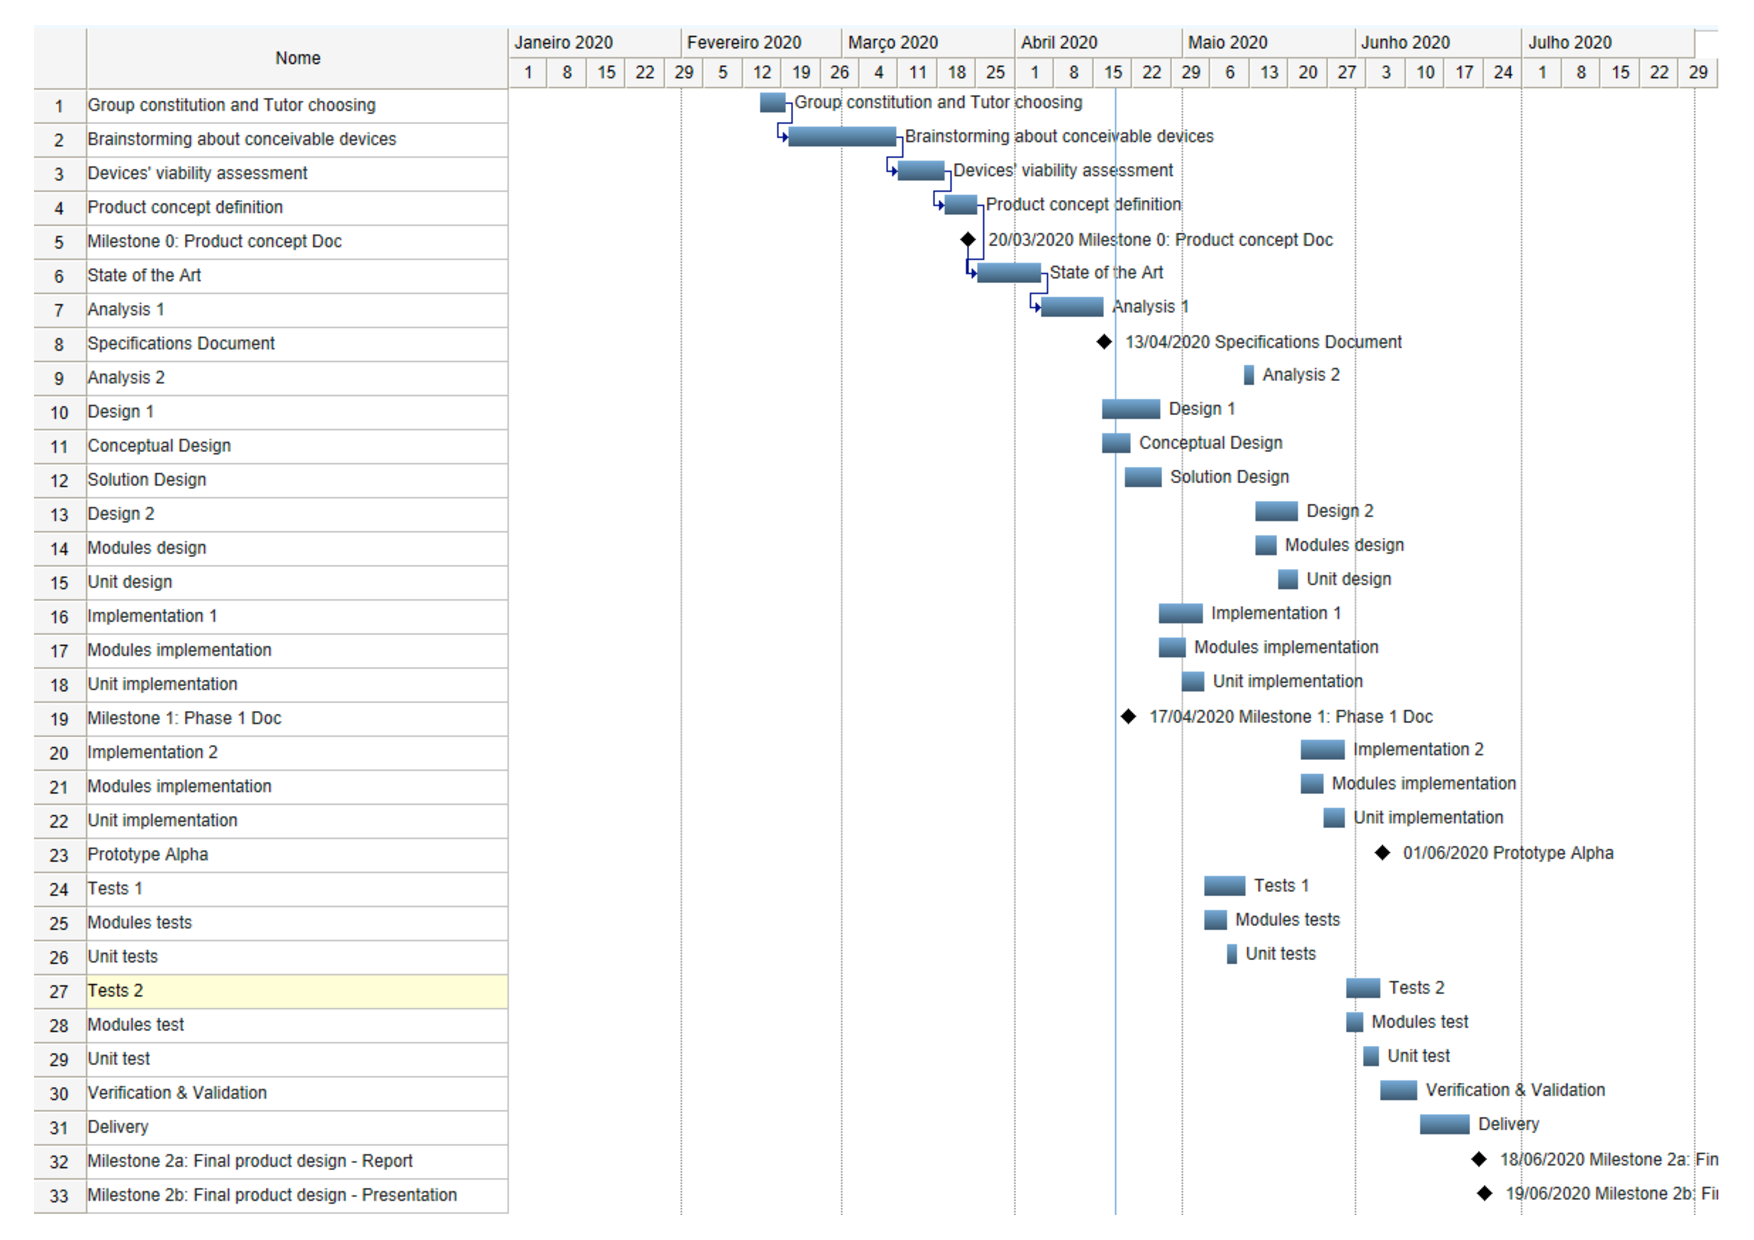
\includegraphics[page=1,width=1.0\textwidth]{sec/pdf/gantt-diag-orig.pdf} 
  \caption{Project planning --- Gantt diagram}%
  \label{fig:gantt-diag-orig}
\end{sidewaysfigure}
% 
%%% Local Variables:
%%% mode: latex
%%% TeX-master: "../../dissertation"
%%% End:

\setcounter{table}{0}
\setcounter{figure}{0}
% the appendix no longer requires the prefix Appendix <Letter>
\chapter{Online Repository --- GitHub}%
\label{ch:append-github}
In Fig.~\ref{fig:github} is illustrated the online repository used to organize the project.\\
 \url{https://github.com/LPI2-DreamTeam/RFCAR}
\begin{figure}[!h]
  \centering
  \includegraphics[width=1.0\textwidth]{./img/append-github.png} 
  \caption{Online Repository --- GitHub}%
  \label{fig:github}
\end{figure}
% 
%%% Local Variables:
%%% mode: latex
%%% TeX-master: "../../dissertation"
%%% End:

\setcounter{table}{0}
\setcounter{figure}{0}
% the appendix no longer requires the prefix Appendix <Letter>
\begin{sidewaysfigure}[!h]
  \centering
  \includegraphics[width=1.0\textwidth]{./img/navig-class-diagram.png} 
  \caption{Navigation subsystem class diagram augmented}%
  \label{fig:navig-class-diagram-augmented}
\end{sidewaysfigure}
% 
%%% Local Variables:
%%% mode: latex
%%% TeX-master: "../../dissertation"
%%% End:

\setcounter{table}{0}
\setcounter{figure}{0}
% the appendix no longer requires the prefix Appendix <Letter>
\begin{sidewaysfigure}[!h]
  \centering
  \includegraphics[width=1.0\textwidth]{./img/smartphone-static-diagram.png} 
  \caption{Smartphone class diagram augmented}%
  \label{fig:uml-android-augmented}
\end{sidewaysfigure}
% 
%%% Local Variables:
%%% mode: latex
%%% TeX-master: "../../dissertation"
%%% End:

\setcounter{table}{0}
\setcounter{figure}{0}
% the appendix no longer requires the prefix Appendix <Letter>
\begin{sidewaysfigure}[!h]
  \centering
  \includegraphics[width=1.0\textwidth]{./img/ClassDiagramVision.png} 
  \caption{Vision Class Diagram augmented}%
  \label{fig:vision-class-diag-augmented}
\end{sidewaysfigure}
% 
%%% Local Variables:
%%% mode: latex
%%% TeX-master: "../../dissertation"
%%% End:

%\setcounter{table}{0}
\setcounter{figure}{0}
% the appendix no longer requires the prefix Appendix <Letter>
\chapter{Use cases (Detailed description)}%
\label{ch:append-UseCases}
In this section, the main use cases are described extensively. As many uses
cases are similar, only changing the parameter to which they refer to, the
Lighting subsystem was used as an example for the Manage<Parameter> use case,
where <Parameter> is Temperature, DoorBell, DateAndTime and SystemNotifications.

\begin{table}
  \captionsetup{justification=raggedright, singlelinecheck=false}
  \caption{Use case LoadGeometryFile}
  \centering
  \begin{tabular}{p{0.26\textwidth}p{0.64\textwidth}}
    \hline
    Use case name & \textbf{LoadGeometryFile} \\ \hline
     Participating actors      & Initiated by the User \\ \hline
     Flow of events & \begin{enum-c}
     \item The User selects the load geometry file option.
     \item The User selects the geometry file to load from a list.
     \item If the file is successfully loaded, the filename is displayed,
       and the file previewed (include \underline{PreviewGeometryFile} use
       case).
     \item Otherwise, an error message is displayed to the user.
     \end{enum-c}\\ \hline 
     Entry conditions       & The User has started the MMSLS machine control
     software and has previously generated a valid geometry file. \\ \hline 
      Exit conditions & The file is successfully loaded, previewed and with the
      filename displayed or an error message is displayed to the User.\\ \hline 
      Quality requirements &  Feedback must be given to the user within 2
      seconds; if files are ``heavy'', display an ongoing processing.\\ \hline 
  \end{tabular}
\label{tab:us-load-geom}
\end{table}

\begin{table}
  \captionsetup{justification=raggedright, singlelinecheck=false}
  \caption{Use case PreviewGeometryFile}
  \centering
  \begin{tabular}{p{0.26\textwidth}p{0.64\textwidth}}
    \hline
    Use case name & \textbf{PreviewGeometryFile} \\ \hline
     Participating actors      & Initiated by the User \\ \hline
     Flow of events & \begin{enum-c}
     \item The User loads the geometry file.
     \item The geometry file is displayed on the canvas.
     \end{enum-c}\\ \hline 
     Entry conditions       & A valid geometry file is loaded into the
     application. \\ \hline 
      Exit conditions & The geometry file is displayed on canvas.      \\ \hline 
      Quality requirements & The preview should be resizable to accommodate
      the various component's dimensions. \\ \hline 
  \end{tabular}
\label{tab:us-prev-geom}
\end{table}

\begin{table}
  \captionsetup{justification=raggedright, singlelinecheck=false}
  \caption{Use case AssignColorsToLaserParams}
  \centering
  \begin{tabular}{p{0.26\textwidth}p{0.64\textwidth}}
    \hline
    Use case name & \textbf{AssignColorsToLaserParams} \\ \hline
     Participating actors      & Initiated by the User \\ \hline
     Flow of events & \begin{enum-c}
     \item The User selects a layer.
     \item The User associates a material's color to its laser's processing color
       counterpart.
     \item The User can edit the laser's processing color attributes.
     \end{enum-c}\\ \hline 
     Entry conditions       & The file is successfully loaded into the
     application and the preview is editable. \\ \hline 
      Exit conditions & The materials' colors has been assigned to valid laser's
      processing color with the respective processing parameters.\\ \hline 
      Quality requirements & Allow multiple line selection. \\ \hline 
  \end{tabular}
\label{tab:us-assign-colors}
\end{table}

\begin{table}
  \captionsetup{justification=raggedright, singlelinecheck=false}
  \caption{Use case LoadManufFile}
  \centering
  \begin{tabular}{p{0.26\textwidth}p{0.64\textwidth}}
    \hline
    Use case name & \textbf{LoadManufFile} \\ \hline
     Participating actors      & Initiated by the User \\ \hline
     Flow of events & \begin{enum-c}
     \item The User selects the load manufacturing file option.
     \item The User selects the manufacturing file to load from a list.
     \item If the file is successfully loaded, the filename is displayed.
     \item Otherwise, an error message is displayed to The User.
     \end{enum-c}\\ \hline 
     Entry conditions       & The User has started the MMSLS machine control
     software and has previously generated a valid manufacturing file. \\ \hline 
      Exit conditions & The file is successfully loaded and with the
      filename displayed or an error message is displayed to the User.      \\ \hline 
      Quality requirements & Feedback must be given to the user within 2
      seconds; if files are 'heavy', display an ongoing processing. \\ \hline 
  \end{tabular}
\label{tab:us-load-manuf}
\end{table}

\begin{table}
  \captionsetup{justification=raggedright, singlelinecheck=false}
  \caption{Use case ConnectToMach}
  \centering
  \begin{tabular}{p{0.26\textwidth}p{0.64\textwidth}}
    \hline
    Use case name & \textbf{ConnectToMach} \\ \hline
     Participating actors      & Initiated by the User \\ \hline
     Flow of events & \begin{enum-c}
     \item The User selects the appropriate connection to the machine from a list.
     \item The User selects the \emph{Connect to Machine} option.
     \item If the connection is successful, the connection status is updated to
       \emph{Connected} and machine operation options are enabled.
     \item Otherwise, an error message is displayed to The User.
     \end{enum-c}\\ \hline 
     Entry conditions       & The User has started the MMSLS machine control
     software and there is physical connection between the \emph{Master} system and
     the \gls{mms}  machine. \\ \hline 
      Exit conditions & The connection is established between \emph{Master} system and
      the \gls{mms} machine or an error message is displayed to the user.\\ \hline 
  \end{tabular}
\label{tab:us-con-to-mach}
\end{table}

\begin{table}
  \captionsetup{justification=raggedright, singlelinecheck=false}
  \caption{Use case DisconnectToMach}
  \centering
  \begin{tabular}{p{0.26\textwidth}p{0.64\textwidth}}
    \hline
    Use case name & \textbf{DisconnectToMach} \\ \hline
     Participating actors      & Initiated by the User \\ \hline
     Flow of events & \begin{enum-c}
     \item The User selects the \emph{Disconnect to Machine} option.
     \item If the disconnection is successful, the connection status is updated to
       \emph{Disconnected} and machine operation options are disabled.
     \item Otherwise, an error message is displayed to The User.
     \end{enum-c}\\ \hline 
     Entry conditions       & A successful connection between the \emph{Master} system
     and the \gls{mms} machine is established.\\ \hline 
      Exit conditions & The connection is closed and the machine operations
      options are disabled or an error messaged is displayed to the user \\ \hline 
  \end{tabular}
\label{tab:us-discon-to-mach}
\end{table}

\begin{table}
  \captionsetup{justification=raggedright, singlelinecheck=false}
  \caption{Use case ManualResetMach}
  \centering
  \begin{tabular}{p{0.26\textwidth}p{0.64\textwidth}}
    \hline
    Use case name & \textbf{ManualResetMach} \\ \hline
     Participating actors      & Initiated by the User \\ \hline
     Flow of events & \begin{enum-c}
     \item The User selects the axis to reset, the direction and the reset
       distance.
     \item When the reset is satisfactory, The User acknowledges this fact by
       selecting the option \emph{Reset end}.
     \item The option to \emph{Start Manufacturing} is now enabled.
     \end{enum-c}\\ \hline 
     Entry conditions       &  A successful connection between the \emph{Master}
     system and the \gls{mms} machine is established.\\ \hline 
      Exit conditions & The reset is satisfactory (User has selected option
      \emph{Reset End}) and the \emph{Start Manufacturing} is enabled.      \\ \hline 
      Quality requirements & Provide feedback to the User of the manual reset
      operations (ascent/descent of the axis) \\ \hline 
  \end{tabular}
\label{tab:us-man-reset}
\end{table}

\begin{table}
  \captionsetup{justification=raggedright, singlelinecheck=false}
  \caption{Use case StartManuf}
  \centering
  \begin{tabular}{p{0.26\textwidth}p{0.64\textwidth}}
    \hline
    Use case name & \textbf{StartManuf} \\ \hline
     Participating actors      & Initiated by the user \\ \hline
     Flow of events & \begin{enum-c}
     \item The User selects the \emph{Start manufacturing} option.
     \item If successful, the machine initiates the manufacturing process
       the machine status is updated to \emph{Run}.
     \end{enum-c}\\ \hline 
     Entry conditions       & \begin{enum-c}
     \item A successful connection between the \emph{Master} system
     and the \gls{mms} machine is established. 
      \item Reset is finished.
      \item Valid geometry and manufacturing file have been loaded.
     \end{enum-c}\\ \hline 
      Exit conditions & \begin{item-c}
      \item \emph{Success}: The \gls{mms} machine status is updated to \emph{Run}, the
        \emph{Start manufacturing} option is disabled, and the options
       \emph{Pause manufacturing} and \emph{Stop manufacturing} are enabled.
     \item \emph{Fail}: An error message is displayed to the user.
      \end{item-c}\\ \hline
      Quality requirements & Update the relevant processing information to the
        User (include use case \underline{UpdateInfo}). \\ \hline 
  \end{tabular}
\label{tab:us-start-manuf}
\end{table}

\begin{table}
  \captionsetup{justification=raggedright, singlelinecheck=false}
  \caption{Use case PauseManuf}
  \centering
  \begin{tabular}{p{0.26\textwidth}p{0.64\textwidth}}
    \hline
    Use case name & \textbf{PauseManuf} \\ \hline
     Participating actors      & Initiated by the user \\ \hline
     Flow of events & \begin{enum-c}
     \item The User selects the \emph{Pause manufacturing} option.
     \item If successful, the manufacturing process is paused.
     \end{enum-c}\\ \hline 
     Entry conditions       & The manufacturing has started (startManuf was
     triggered), but has not yet finished. \\ \hline 
      Exit conditions & \begin{item-c}
      \item \emph{Success}: The manufacturing process is paused, and
        the \gls{mms} machine status is updated to \emph{Idle}. The \emph{Pause
        manufacturing} option is disabled and the \emph{Start manufacturing}
        option is re-enabled.
     \item \emph{Fail}: An error message is displayed to the user.
      \end{item-c}\\ \hline
  \end{tabular}
\label{tab:us-pause-manuf}
\end{table}

\begin{table}
  \captionsetup{justification=raggedright, singlelinecheck=false}
  \caption{Use case StopManuf}
  \centering
  \begin{tabular}{p{0.26\textwidth}p{0.64\textwidth}}
    \hline
    Use case name & \textbf{StopManuf} \\ \hline
     Participating actors      & Initiated by the User \\ \hline
     Flow of events & \begin{enum-c}
     \item The User selects the \emph{Stop manufacturing} option.
     \item If successful, the manufacturing process is stopped.
     \end{enum-c}\\ \hline 
     Entry conditions & The manufacturing has started (startManuf was
     triggered), but has not yet finished. \\ \hline 
      Exit conditions & \begin{item-c}
      \item \emph{Success}: The manufacturing process is stopped, and
        the \gls{mms} machine status is updated to \emph{Stopped}. The
        \emph{Stop manufacturing} option is disabled and the \emph{Start
        manufacturing} option is re-enabled.
     \item \emph{Fail}: An error message is displayed to the user.
      \end{item-c}\\ \hline
  \end{tabular}
\label{tab:us-stop-manuf}
\end{table}

Although several notifications from relevant events are to be notified by the
\emph{Master} machine to the User, for brevity purposes only the most relevant one is
showcased here, namely \underline{NotifyManufEnd}.

\begin{table}
  \captionsetup{justification=raggedright, singlelinecheck=false}
  \caption{Use case NotifyManufEnd}
  \centering
  \begin{tabular}{p{0.26\textwidth}p{0.64\textwidth}}
    \hline
    Use case name & \textbf{NotifyManufEnd} \\ \hline
     Participating actors      & Initiated by MMS-Mach; User participates \\ \hline
     Flow of events & \begin{enum-c}
     \item When manufacturing is completed, the \emph{Master} system notifies The User
       about this fact.
     \end{enum-c}\\ \hline 
     Entry conditions & The manufacturing has started (startManuf was
     triggered), and is not paused or stopped. \\ \hline 
     Exit conditions & The manufacturing process stops and the User is notified
      about this fact.\\ \hline 
  \end{tabular}
\label{tab:us-notif-manuf-end}
\end{table}

\begin{table}[!hbt]
  \captionsetup{justification=raggedright, singlelinecheck=false}
  \caption{Use case VisualizeManuf}
  \centering
  \begin{tabular}{p{0.26\textwidth}p{0.64\textwidth}}
    \hline
    Use case name & \textbf{VisualizeManuf} \\ \hline
     Participating actors      & Initiated by MMS-Mach or Laser; User participates \\ \hline
     Flow of events & \begin{enum-c}
     \item Relevant manufacturing information is sent by the MMS-Mach or the
       Laser to the \emph{Master} system --- on a time-basis or triggered by a
       relevant event like the manufacturing completion of one layer --- that is
       updated to the User.
     \end{enum-c}\\ \hline 
     Entry conditions & The manufacturing has started (startManuf was
     triggered)\\ \hline
      Exit conditions & The manufacturing is stopped or has ended. \\ \hline 
      Quality requirements & \begin{item-c}
      \item \emph{Time-basis} The relevant manufacturing information must be
        updated with 1 second refresh rate.
      \item \emph{Event} The information associated with the triggering event
        must be updated immediately.
      \end{item-c} \\ \hline 
  \end{tabular}
\label{tab:vis-manuf}
\end{table}

%%% Local Variables:
%%% mode: latex
%%% TeX-master: "../../dissertation"
%%% End:

%\setcounter{table}{0}
\setcounter{figure}{0}
%
\chapter{Sequence Diagrams}
\label{ch:append-seq-diag}
\begin{figure*}
  \begin{center}
    \includegraphics[height=1.0\textheight]{./img/seq-start-manuf-lscape.png}
  \end{center}
  \caption{Sequence diagram for the \emph{StartManuf} use case (Part 1)}\label{fig:seq-start-manuf-lscape}
\end{figure*}

\begin{figure*}
  \begin{center}
    \includegraphics[height=1.0\textheight]{./img/seq-start-process-lscape.png}
  \end{center}
  \caption{Sequence diagram for the \emph{StartManuf} use case (Part 2)}\label{fig:seq-start-process-lscape}
\end{figure*}
%
%\clearpage
%
%% src:https://www.reddit.com/r/LaTeX/comments/4jynr7/adding_a3_pdf_page_into_an_a4_document/d3ba7eg/ 
%\KOMAoptions{paper=A3,pagesize}
%%\KOMAoptions{paper=landscape, pagesize}
%
%\label{ch:append-UseCases}
%\begin{figure*}
%  \begin{center}
%    \includegraphics[width=1.6\textwidth]{./img/seq-start-manuf.png}
%  \end{center}
%  \caption{Sequence diagram for the \emph{StartManuf} use case (Part 1)}%
%\label{fig:seq-start-manufA3}
%\end{figure*}
%
%\begin{figure*}
%  \begin{center}
%    \includegraphics[width=1.6\textwidth]{./img/seq-start-process.png}
%  \end{center}
%  \caption{Sequence diagram for the \emph{StartManuf} use case (Part 2)}%
%\label{fig:seq-start-processA3}
%\end{figure*}
%
%\cleardoublepage
%\KOMAoptions{paper=A4, pagesize}

%
%%% Local Variables:
%%% mode: latex
%%% TeX-master: "../../dissertation"
%%% End:

%
	%\chapter{Support material}
	%Auxiliary results which are not main-stream; or
%
	%\chapter{Details of results}
	%Details of results whose length would compromise readability of main text; or
%
	%\chapter{Listings}
	%Specifications and Code Listings: should this be the case; or
%
	%\chapter{Tooling}
	%Tooling: Should this be the case.
%
	%Anyone using \Latex\ should consider having a look at \TUG,
	%the \tug{\TeX\ Users Group}
%
	% Back Cover -------------------------------------------
%	\umbackcover{
%%	NB: place here information about funding, FCT project, etc in which the
%%	work is framed. Leave empty otherwise.
%         % The author gratefully acknowledges the financial support of ``Fundação
%         % para a Ciência e Tecnologia'' (FCT – Portugal), through the research
%         % project PTDC/ECM/108146/2008 (“Generalised Beam Theory (GBT) –
%         % Development, Application and Dissemination”).
%         % HAMaBICo --- Hybrid Additive Manufacturing for Bio Inspired Component
%         % through the research project  NORTE-01-0145-FEDER-000018.
%          The author gratefully acknowledges the financial support of this
%          project through the research projects NORTE-01-0145-FEDER-000018
%          (HAMaBICo --- Hybrid Additive Manufacturing for Bio Inspired
%          Component) and POCI-01-0145-FEDER-030498 (FunImp --- Design and
%          Fabrication of MultiFunctional Implants).
%	}
\end{document}
%%% Local Variables:
%%% mode: latex
%%% TeX-master: t
%%% End: